\documentclass[12pt,a4paper]{article}

\usepackage{xeCJK}
\usepackage{amsmath,amsthm,amssymb}
\usepackage[colorlinks,linkcolor=blue]{hyperref}
\usepackage{graphicx}
\usepackage{xcolor}
\usepackage{float}
\usepackage{makeidx}
\usepackage{listings} 
\usepackage[numbers,sort&compress]{natbib}
\usepackage[level]{datetime}
\usepackage{indentfirst}
\usepackage{enumitem}
\usepackage{draftwatermark}
\usepackage{titlesec}
\usepackage{fancyhdr}
\usepackage[top=1.5cm, bottom=2cm, outer=1.5cm, inner=1.5cm, heightrounded, marginparwidth=0cm, marginparsep=0cm]{geometry}
%\usepackage{showframe}

\renewcommand{\today}{\number\year 年 \number\month 月 \number\day 日}
\renewcommand{\refname}{参考文献}
\renewcommand{\tablename}{表}
\renewcommand{\contentsname}{目录}

\newcommand{\upcite}[1]{\textsuperscript{\textsuperscript{\cite{#1}}}}
\newcommand{\tabincell}[2]{\begin{tabular}{@{}#1@{}}#2\end{tabular}}

\definecolor{dkgreen}{rgb}{0,0.6,0}
\definecolor{gray}{rgb}{0.5,0.5,0.5}
\definecolor{mauve}{rgb}{0.58,0,0.82}
\lstset{
  language=c++, 
  basicstyle=\footnotesize,  
  % numbers=left,      
  numberstyle=\tiny\color{gray}, 
  stepnumber=2, 
  numbersep=5pt,
  backgroundcolor={},
  showspaces=false,   
  showstringspaces=false,
  showtabs=false,         
  frame=single,                   % frame around code [single, shadowbox]
  rulecolor=\color{black}, 
  tabsize=2,                     
  captionpos=b,                   % caption-position bottom
  breaklines=true,                % automatic line breaking
  breakatwhitespace=false, 
  % title=\lstname,               % filename included with \lstinputlisting;
  keywordstyle=\color{blue},     
  commentstyle=\color{dkgreen}, 
  stringstyle=\color{mauve},     
  escapeinside={\%*}{*)},         % if want to add LaTeX within your code
  morekeywords={*,...}            % if want to add more keywords to the set
}

\SetWatermarkText{\textsc{CGGOS}}
\SetWatermarkScale{1}
%\SetWatermarkFontSize{4cm}
%\SetWatermarkLightness{0.5}

%\newpagestyle{main}{            
%  \sethead{}{VINS-Mono 论文公式推导与代码解析}{\url{https://cggos.github.io}}
%  \headrule
%  \setfoot{}{}{}
%%  \footrule
%}
%\pagestyle{main} 

\pagestyle{fancy}
\lhead{}
\chead{VINS-Mono 论文公式推导与代码解析}
\rhead{}
\lfoot{更新于 \date{\today}}
\cfoot{\thepage}
\rfoot{\url{https://github.com/cggos}}
\renewcommand{\headrulewidth}{0.4pt}
\renewcommand{\footrulewidth}{0.4pt}

\bibliographystyle{unsrt}

\title{VINS-Mono 论文公式推导与代码解析}
\author{高洪臣}
\date{2019年3月16日}


\begin{document}

\maketitle
\tableofcontents

\noindent
\setlength{\parindent}{2em}
\setlength{\parskip}{0.3em}
\linespread{1}

\section{概述} 

\begin{figure}[htbp]
\centering
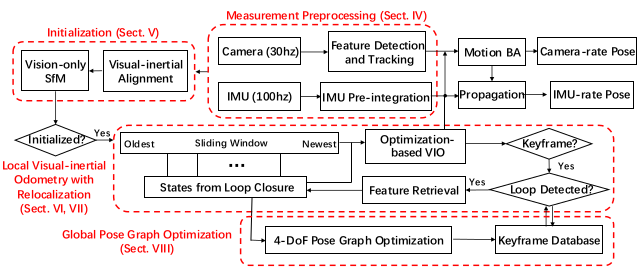
\includegraphics[scale=0.6]{images/vins_mono_framework.png}
\end{figure}

\textbf{Monocular visual-inertial odometry} with relocalization achieved via nonlinear graph optimization-based, tightly-coupled, sliding window, visual-inertial bundle adjustment. \cite{qin2017vins}

代码(注释版): \href{https://github.com/cggos/vins_mono_cg}{cggos/vins\_mono\_cg} 

\section{测量预处理} 

\subsection{前端视觉处理}

\begin{itemize}

  \item Simple feature processing pipeline
  \item 自适应直方图均衡化(\verb|cv::CLAHE|)
  \item 掩模处理,特征点均匀分布(\verb|setMask|)
  \item 提取图像Harris角点(\verb|cv::goodFeaturesToTrack|)
  \item KLT金字塔光流跟踪(\verb|cv::calcOpticalFlowPyrLK|)
  \item 连续帧跟踪
  \item 基础矩阵(RANSAC)去除外点(\verb|rejectWithF|)
  \item 发布 \verb|feature_points(id_of_point, un_pts, cur_pts, pts_velocity)|
  \item Keyframe selection
  
  \begin{itemize}
  \item Case 1: Rotation-compensated average feature parallax is larger than a threshold
  \item Case 2: Number of tracked features in the current frame is less than a threshold
  \item All frames are used for optimization, but non-keyframes are removed first
  \end{itemize}  
  
\end{itemize}  

\subsection{IMU 预积分}

\begin{figure}[htbp]
\centering
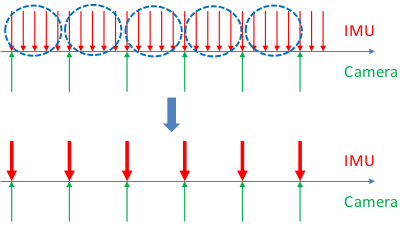
\includegraphics[scale=0.6]{images/imu_integration_01.png}
\end{figure}

\subsubsection{IMU 测量方程}

忽略地球自转,IMU测量方程为

\begin{equation}
\begin{aligned} 
\hat{\mathbf{a}}_{t} 
&= 
\mathbf{a}_{t}+\mathbf{b}_{a_{t}}+\mathbf{R}_{w}^{t} \mathbf{g}^{w}+\mathbf{n}_{a} \\ 
\hat{\boldsymbol{\omega}}_{t} 
&=
\boldsymbol{\omega}_{t}+\mathbf{b}_{w_{t}}+\mathbf{n}_{w} 
\end{aligned}
\end{equation}

\subsubsection{预积分方程}

(1)\textbf{IMU integration in world frame}

由上面的IMU测量方程积分就可以计算出下一时刻的p、v和q:  

\begin{equation}
\begin{aligned} 
\mathbf{p}_{b_{k+1}}^{w}&=
\mathbf{p}_{b_{k}}^{w} + \mathbf{v}_{b_{k}}^{w} \Delta t_{k} + \iint_{t \in\left[t_{k}, t_{k+1}\right]}\left(\mathbf{R}_{t}^{w}\left(\hat{\mathbf{a}}_{t}-\mathbf{b}_{a_{t}}-\mathbf{n}_{a}\right)-\mathbf{g}^{w}\right) d t^{2} \\ 
\mathbf{v}_{b_{k+1}}^{w}&=
\mathbf{v}_{b_{k}}^{w}+\int_{t \in\left[t_{k}, t_{k+1}\right]}\left(\mathbf{R}_{t}^{w}\left(\hat{\mathbf{a}}_{t}-\mathbf{b}_{a_{t}}-\mathbf{n}_{a}\right)-\mathbf{g}^{w}\right) d t \\
\mathbf{q}_{b_{k+1}}^{w}&=
\mathbf{q}_{b_{k}}^{w} \otimes \int_{t \in\left[t_{k}, t_{k+1}\right]} \frac{1}{2} \boldsymbol{\Omega}\left(\hat{\boldsymbol{\omega}}_{t}-\mathbf{b}_{w_{t}}-\mathbf{n}_{w}\right) \mathbf{q}_{t}^{b_{k}} d t
\end{aligned}
\end{equation}

其中,

\begin{equation}
\boldsymbol{\Omega}(\boldsymbol{\omega}) =
\left[\begin{array}{c}
\boldsymbol{\omega} \\ 0
\end{array}\right]_{R} = 
\left[\begin{array}{cc}
{-\lfloor\boldsymbol{\omega}\rfloor_{ \times}} & {\boldsymbol{\omega}} \\ 
{-\boldsymbol{\omega}^{T}} & {0}
\end{array}\right], \quad
\lfloor\boldsymbol{\omega}\rfloor_{ \times}=
\left[\begin{array}{ccc}
{0} & {-\omega_{z}} & {\omega_{y}} \\ 
{\omega_{z}} & {0} & {-\omega_{x}} \\ 
{-\omega_{y}} & {\omega_{x}} & {0}
\end{array}\right]
\end{equation}

(2)\textbf{IMU integration in the body frame of first pose of interests}

\begin{figure}[htbp]
\centering
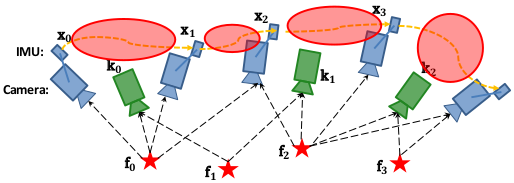
\includegraphics[scale=0.6]{images/imu_integration_02.png}
\end{figure}

为避免重新传播IMU观测值,选用IMU预积分模型,从世界坐标系转为本体坐标系

\begin{equation}
\begin{aligned} 
\mathbf{R}_{w}^{b_{k}} \mathbf{p}_{b_{k+1}}^{w} &=
\mathbf{R}_{w}^{b_{k}}\left(\mathbf{p}_{b_{k}}^{w}+\mathbf{v}_{b_{k}}^{w} \Delta t_{k}-\frac{1}{2} \mathbf{g}^{w} \Delta t_{k}^{2}\right)+\boldsymbol{\alpha}_{b_{k+1}}^{b_{k}} \\ 
\mathbf{R}_{w}^{b_{k}} \mathbf{v}_{b_{k+1}}^{w} &=
\mathbf{R}_{w}^{b_{k}}\left(\mathbf{v}_{b_{k}}^{w}-\mathbf{g}^{w} \Delta t_{k}\right)+\boldsymbol{\beta}_{b_{k+1}}^{b_{k}} \\ 
\mathbf{q}_{w}^{b_{k}} \otimes \mathbf{q}_{b_{k+1}}^{w} &=
\boldsymbol{\gamma}_{b_{k+1}}^{b_{k}} 
\end{aligned}
\end{equation}

则 IMU预积分模型(\textbf{预积分估计值})为

\begin{equation}
\label{equ:preinte_estimate}
\left[\begin{array}{c}
{\hat{\boldsymbol{\alpha}}_{b_{k+1}}^{b_{k}}} \\ 
{\hat{\boldsymbol{\beta}}_{b_{k+1}}^{b_{k}}}  \\ 
{\hat{\boldsymbol{\gamma}}_{b_{k+1}}^{b_{k}+1}} \\ 
{\mathbf{0}} \\ 
{\mathbf{0}}
\end{array}\right]=
\left[\begin{array}{c}
{\mathbf{R}_{w}^{b_{k}}\left(\mathbf{p}_{b_{k+1}}^{w}-\mathbf{p}_{b_{k}}^{w}+\frac{1}{2} \mathbf{g}^{w} \Delta t_{k}^{2}-\mathbf{v}_{b_{k}}^{w} \Delta t_{k}\right)} \\
{\mathbf{R}_{w}^{b_{k}}\left(\mathbf{v}_{b_{k+1}}^{w}+\mathbf{g}^{w} \Delta t_{k}-\mathbf{v}_{b_{k}}^{w}\right)} \\ 
{\mathbf{q}_{b_{k}}^{w_{k}} \otimes \mathbf{q}_{b_{k+1}}} \\ 
{\mathbf{b}_{a b_{k+1}}-\mathbf{b}_{a b_{k}}} \\ 
{\mathbf{b}_{w b_{k+1}}-\mathbf{b}_{w b_{k}}}
\end{array}\right]
\end{equation}


离散状态下采用 \textbf{中值积分(mid-point)} 的预积分方程(\textbf{预积分测量值})为

\begin{equation}
\label{equ:preinte_measure}
\begin{cases}
\begin{aligned}
\color{blue}{\delta \mathbf{q}_{i+1}} &= 
\delta \mathbf{q}_{i} \otimes 
\begin{bmatrix} 1 \\ \frac{1}{2} \boldsymbol{\omega}_{i}^{\prime} \delta t \end{bmatrix} \\
\color{blue}{\delta \boldsymbol{\alpha}_{i+1}} &= 
\delta \boldsymbol{\alpha}_{i} + \delta \boldsymbol{\beta}_{i}t + \frac{1}{2} \mathbf{a}_{i}^{\prime} \delta t^{2} \\
\color{blue}{\delta \boldsymbol{\beta}_{i+1}} &= 
\delta \boldsymbol{\beta}_{i}+\mathbf{a}_{i}^{\prime} \delta t \\
{\mathbf{b}_a}_{i+1} &= {\mathbf{b}_a}_i + \mathbf{n}_{ba} \delta t \\
{\mathbf{b}_g}_{i+1} &= {\mathbf{b}_g}_i + \mathbf{n}_{bg} \delta t
\end{aligned}
\end{cases}
\end{equation}

其中

\begin{equation}
\begin{aligned}
\boldsymbol{\omega}_{i}' 
&= 
\frac{(\boldsymbol{\omega}_i-{\mathbf{b}_g}_i+{\mathbf{n}_w}_0)+(\boldsymbol{\omega}_{i+1}-{\mathbf{b}_g}_i+{\mathbf{n}_w}_1)}{2} \\
&= 
\frac{\boldsymbol{\omega}_{i+1}+\boldsymbol{\omega}_{i}+{\mathbf{n}_w}_0+{\mathbf{n}_w}_1}{2}-{\mathbf{b}_g}_i \\
\mathbf{a}_{i}' 
&= 
\frac{\delta \mathbf{q}_{i} (\mathbf{a}_{i}-{\mathbf{b}_a}_i+{\mathbf{n}_a}_0)+
{\color{blue}{\delta \mathbf{q}_{i+1}}}(\mathbf{a}_{i+1}-{\mathbf{b}_a}_i+{\mathbf{n}_a}_1)}{2}
\end{aligned}
\end{equation}

\verb|midPointIntegration| 中的相关代码(没有考虑噪声):  

\begin{lstlisting}
Vector3d un_gyr = 0.5 * (_gyr_0 + _gyr_1) - linearized_bg;
result_delta_q  = 
  delta_q * Quaterniond(1, un_gyr(0)*_dt/2, un_gyr(1)*_dt/2, un_gyr(2)*_dt/2);

Vector3d un_acc_0 =        delta_q * (_acc_0 - linearized_ba);
Vector3d un_acc_1 = result_delta_q * (_acc_1 - linearized_ba);
Vector3d un_acc   = 0.5 * (un_acc_0 + un_acc_1);

result_delta_p = delta_p + delta_v * _dt + 0.5 * un_acc * _dt * _dt;
result_delta_v = delta_v + un_acc * _dt;

// 预积分的过程中Bias没有发生改变
result_linearized_ba = linearized_ba;
result_linearized_bg = linearized_bg;
\end{lstlisting}

\subsubsection{误差状态方程}

IMU(预积分)误差状态向量  

\begin{equation}
\delta \mathcal{X} =
[
\delta \mathbf{P} \quad 
\delta \boldsymbol{\theta} \quad 
\delta \mathbf{v} \quad 
\delta \mathbf{b}_a \quad 
\delta \mathbf{b}_g]^T
\in \mathbb{R}^{15 \times 1}
\end{equation}

根据 \cite{DBLP:journals/corr/abs-1711-02508} ESKF 中 \textit{\textbf{5.3.3 The error-state kinematics}} 小节公式  

\begin{equation}
\begin{aligned}
\dot{\delta \mathbf{p}} &= \delta \mathbf{v} \\
\dot{\delta \mathbf{v}} &= -\mathbf{R}\left[\mathbf{a}_{m}-\mathbf{a}_{b}\right]_{ \times} \delta \boldsymbol{\theta}-\mathbf{R} \delta \mathbf{a}_{b}+\delta \mathbf{g}-\mathbf{R} \mathbf{a}_{n} \\
\dot{\delta \boldsymbol{\theta}} &= -\left[\boldsymbol{\omega}_{m}-\boldsymbol{\omega}_{b}\right]_{ \times} \delta \boldsymbol{\theta}-\delta \boldsymbol{\omega}_{b}-\boldsymbol{\omega}_{n} \\
\delta \dot{\mathbf{a}}_{b} &= \mathbf{a}_{w} \\ 
\delta \dot{\boldsymbol{\omega}}_{b} &= \boldsymbol{\omega}_{w} \\ 
\dot{\delta \mathbf{g}} &= 0 
\end{aligned}
\end{equation}

对于 \textbf{中值积分(mid-point)} 下的 \textbf{误差状态方程的导数} 为  

\begin{equation}
\dot{\delta X_k} =
\begin{cases}
\dot{\delta \theta_{k}} =&
-[\frac{w_{k+1}+w_{k}}{2}-b_{g_{k}}]_{\times} \delta \theta_{k}-\delta b_{g_{k}}+\frac{n_{w0}+n_{w1}}{2} \\
\dot{\delta\beta_{k}} =&
-\frac{1}{2}q_{k}[a_{k}-b_{a_{k}}]_{\times}\delta \theta \\
&-\frac{1}{2}q_{k+1}[a_{k+1}-b_{a_{k}}]_{\times}((I-[\frac{w_{k+1}+w_{k}}{2}-b_{g_{k}}]_{\times }\delta t) \delta \theta_{k} -\delta b_{g_{k}}\delta t+\frac{n_{w0}+n_{w1}}{2}\delta t) \\
&-\frac{1}{2}q_{k}\delta b_{a_{k}}-\frac{1}{2}q_{k+1}\delta b_{a_{k}}-\frac{1}{2}q_{k}n_{a0}-\frac{1}{2}q_{k}n_{a1} \\
\dot{\delta\alpha_{k}} =&
-\frac{1}{4}q_{k}[a_{k}-b_{a_{k}}]_{\times}\delta \theta\delta t \\
&-\frac{1}{4}q_{k+1}[a_{k+1}-b_{a_{k}}]_{\times}((I-[\frac{w_{k+1}+w_{k}}{2}-b_{g_{k}}]_{\times }\delta t) \delta \theta _{k} -\delta b_{g_{k}}\delta t+\frac{n_{w0}+n_{w1}}{2}\delta t)\delta t \\
&-\frac{1}{4}q_{k}\delta b_{a_{k}}\delta t-\frac{1}{4}q_{k+1}\delta b_{a_{k}}\delta t-\frac{1}{4}q_{k}n_{a0}\delta t-\frac{1}{4}q_{k}n_{a1}\delta t \\
\dot{\delta b_{a_k}} =&  n_{b_a} \\
\dot{\delta b_{g_k}} =&  n_{b_g}
\end{cases}
\end{equation}

则\textbf{IMU预积分(误差)状态方程}为

\begin{equation}
\dot{\delta \mathbf{X}_k} = \mathbf{F} \delta \mathbf{X}_k + \mathbf{G} \mathbf{n}
\end{equation}

则 IMU预积分状态传递方程 为

\begin{equation}
\label{equ:preinte_iter_time}
\begin{aligned}
\delta X_{k+1}
&= \delta X_k + \dot{\delta X_k} \delta t \\
&= \delta X_k + (F \delta X_k + Gn) \delta t \\
&= (I + F \delta t) \delta X_k + (G \delta t) n
\end{aligned}
\end{equation}

令

\begin{equation}
\label{equ:F1_G1}
\begin{aligned}
F' &= I + F \delta t &\in \mathbb{R}^{15 \times 15} \\
G' &= G \delta t     &\in \mathbb{R}^{15 \times 18}
\end{aligned}
\end{equation}

最终,\textbf{IMU预积分递推方程}为

\begin{equation}
\label{equ:preinte_iter_simple}
\delta \mathbf{X}_{k+1} 
= \mathbf{F}^{\prime} \delta \mathbf{X}_k + \mathbf{G}^{\prime} \mathbf{n}
\end{equation}

式\eqref{equ:preinte_iter_simple} 展开得

\begin{equation}
\label{equ:preinte_iter_complete}
\begin{aligned}
\begin{bmatrix}
\delta \alpha_{k+1} \\
\delta \theta_{k+1} \\
\delta \beta_{k+1} \\
\delta b_{a{}{k+1}} \\
\delta b_{g{}{k+1}}
\end{bmatrix} =&
\begin{bmatrix}
I & f_{12} & I\delta t & -\frac{1}{4}(q_{k}+q_{k+1})\delta t^{2} & f_{15} \\
0 & I-[\frac{w_{k+1}+w_{k}}{2}-b_{wk}]_{\times } \delta t & 0 & 0 & -I\delta t \\
0 & f_{32} & I & -\frac{1}{2}(q_{k}+q_{k+1})\delta t & f_{35} \\
0 & 0 & 0 & I & 0 \\
0 & 0 & 0 & 0 & I
\end{bmatrix}
\begin{bmatrix}
\delta \alpha_{k} \\
\delta \theta_{k} \\
\delta \beta_{k} \\
\delta b_{a{}{k}} \\
\delta b_{g{}{k}}
\end{bmatrix} \\
+&
\begin{bmatrix}
\frac{1}{4}q_{k}\delta t^{2} & g_{12} & \frac{1}{4}q_{k+1}\delta t^{2} & g_{14} & 0 & 0 \\
0 & \frac{1}{2}I\delta t & 0 & \frac{1}{2}I\delta t & 0 & 0 \\
\frac{1}{2}q_{k}\delta t & g_{32} & \frac{1}{2}q_{k+1}\delta t & g_{34} & 0 & 0 \\
0 & 0 & 0 & 0 & I\delta t & 0 \\
0 & 0 & 0 & 0 & 0 & I\delta t
\end{bmatrix}
\begin{bmatrix}
n_{a0}\\
n_{w0}\\
n_{a1}\\
n_{w1}\\
n_{ba}\\
n_{bg}
\end{bmatrix}
\end{aligned}
\end{equation}

其中,

\begin{equation}
\begin{cases}
\begin{aligned}
f_{12} &= \frac{\partial{\alpha_{k+1}}}{\partial{\delta \theta_k}} = 
-\frac{1}{4}q_{k}[a_{k}-b_{a_{k}}]_{\times}\delta t^{2}-\frac{1}{4}q_{k+1}[a_{k+1}-b_{a_{k}}]_{\times}(I-[\frac{w_{k+1}+w_{k}}{2}-b_{g_{k}}]_{\times }\delta t)\delta t^{2} \\
f_{32} &= \frac{\partial{\beta_{k+1}}}{\partial{\delta \theta_k}} =
-\frac{1}{2}q_{k}[a_{k}-b_{a_{k}}]_{\times}\delta t-\frac{1}{2}q_{k+1}[a_{k+1}-b_{a_{k}}]_{\times}(I-[\frac{w_{k+1}+w_{k}}{2}-b_{g_{k}}]_{\times }\delta t)\delta t \\
f_{15} &= \frac{\partial{\alpha_{k+1}}}{\partial{\delta {b_g}_k}} =
\frac{1}{4}(-q_{k+1}[a_{k+1}-b_{a_{k}}]_{\times}\delta t^{2})(-\delta t) \\
f_{35} &= \frac{\partial{\beta_{k+1}}}{\partial{\delta {b_g}_k}} =
\frac{1}{2}(-q_{k+1}[a_{k+1}-b_{a_{k}}]_{\times}\delta t)(-\delta t) \\
g_{12} &= \frac{\partial{\alpha_{k+1}}}{\partial{{n_g}_0}} = 
\frac{1}{4}(-q_{k+1}[a_{k+1}-b_{a_{k}}]_{\times}\delta t^{2})\frac{1}{2}\delta t \\
g_{14} &= \frac{\partial{\alpha_{k+1}}}{\partial{{n_g}_1}} = 
\frac{1}{4}(-q_{k+1}[a_{k+1}-b_{a_{k}}]_{\times}\delta t^{2})\frac{1}{2}\delta t \\
g_{32} &= \frac{\partial{\beta_{k+1}}}{\partial{{n_g}_0}} =
\frac{1}{2}(-q_{k+1}[a_{k+1}-b_{a_{k}}]_{\times}\delta t^{2})\frac{1}{2}\delta t \\
g_{34} &= \frac{\partial{\beta_{k+1}}}{\partial{{n_g}_1}} =
\frac{1}{2}(-q_{k+1}[a_{k+1}-b_{a_{k}}]_{\times}\delta t^{2})\frac{1}{2}\delta t
\end{aligned}
\end{cases}
\end{equation}

式\eqref{equ:F1_G1}\eqref{equ:preinte_iter_simple}中的 $F'$ 即代码中 \verb|F|,$G'$ 即代码中 \verb|V|,相关代码见 \verb|midPointIntegration|。

另外,状态误差传递的线性递推关系可通过两种方法实现:

\begin{itemize}[itemindent=1em]
  \item \textbf{基于误差随时间变化的递推方程}
  \item \textbf{基于一阶泰勒展开的误差递推方程}
\end{itemize}

上面式\eqref{equ:preinte_iter_simple} $F'$ 和 $G'$ 的计算是用的第一种方法;我们还可以通过第二种方法:已知IMU预积分(中值积分)测量方程\eqref{equ:preinte_measure},将其表示成式\eqref{equ:preinte_iter_simple}的形式(其中,$F'$是状态量$\delta X_{k+1}$对状态量$\delta X_k$的雅克比矩阵,$G'$是状态量$\delta X_{k+1}$对输入量$n_{k-1}$的雅克比矩阵),通过求导计算出 $F'$ 和 $G'$。

最后,计算

\begin{itemize}[itemindent=1em]
  \item IMU预积分测量关于IMU Bias 的 \textbf{雅克比矩阵} $\mathbf{J}_{k+1}$
  \item IMU预积分测量的 \textbf{协方差矩阵} $\mathbf{P}_{k+1}$
  \item 噪声的 \textbf{协方差矩阵} $\mathbf{Q}$
\end{itemize}

雅克比矩阵的传递方程为

\begin{equation}
\mathbf{J}_{b_k} = \mathbf{I}_{15 \times 15}
\end{equation}

\begin{equation}
\begin{aligned}
\mathbf{J}_{t+\delta t} 
&= 
\mathbf{F^{\prime}} \mathbf{J}_t \\
&= 
(\mathbf{I} + \mathbf{F}_t \delta t) \mathbf{J}_t, \quad t \in [k, k+1]
\end{aligned}
\end{equation}

协方差矩阵的传递方程为

\begin{equation}
\mathbf{P}_{b_{k}}^{b_k} = \mathbf{0}_{15 \times 15}
\end{equation}

\begin{equation}
\begin{aligned}
\mathbf{P}_{t+\delta t}^{b_k} 
&= 
F' P_t^{b_k} F'^T + G' Q {G'}^T \\
&= 
(I + F_t \delta t)P_{t}^{b_k}(I + F_t \delta t)^T + (G_t \delta t)Q(G_t \delta t)^T
\end{aligned}
\end{equation}

其中,噪声协方差矩阵为

\begin{equation}
\mathbf{Q} = 
\text{diag}(
  \sigma_{a_0}^2 \quad \sigma_{\omega_0}^2 \quad
  \sigma_{a_1}^2 \quad \sigma_{\omega_1}^2 \quad
  \sigma_{b_a}^2 \quad \sigma_{b_g}^2) 
\in \mathbb{R}^{18 \times 18}
\end{equation}

\begin{lstlisting}
ACC_N = fsSettings["acc_n"];  ACC_W = fsSettings["acc_w"];
GYR_N = fsSettings["gyr_n"];  GYR_W = fsSettings["gyr_w"];

noise = Eigen::Matrix<double, 18, 18>::Zero();
noise.block<3, 3>(0, 0)   =  (ACC_N * ACC_N) * Eigen::Matrix3d::Identity();
noise.block<3, 3>(3, 3)   =  (GYR_N * GYR_N) * Eigen::Matrix3d::Identity();
noise.block<3, 3>(6, 6)   =  (ACC_N * ACC_N) * Eigen::Matrix3d::Identity();
noise.block<3, 3>(9, 9)   =  (GYR_N * GYR_N) * Eigen::Matrix3d::Identity();
noise.block<3, 3>(12, 12) =  (ACC_W * ACC_W) * Eigen::Matrix3d::Identity();
noise.block<3, 3>(15, 15) =  (GYR_W * GYR_W) * Eigen::Matrix3d::Identity();
\end{lstlisting}

当bias估计轻微改变时,我们可以使用如下的一阶近似 \textbf{对中值积分得到的预积分测量值进行矫正},而\textbf{不重传播},从而得到 \textbf{更加精确的预积分测量值}(bias修正的线性模型)

\begin{equation}
\begin{aligned} 
\boldsymbol{\alpha}_{b_{k+1}}^{b_{k}} & \approx 
\hat{\boldsymbol{\alpha}}_{b_{k+1}}^{b_{k}}+
\mathbf{J}_{b_{a}}^{\alpha} \delta \mathbf{b}_{a_{k}}+
\mathbf{J}_{b_{w}}^{\alpha} \delta \mathbf{b}_{w_{k}} \\ 
\boldsymbol{\beta}_{b_{k+1}}^{b_{k}} & \approx 
\hat{\boldsymbol{\beta}}_{b_{k+1}}^{b_{k}}+
\mathbf{J}_{b_{a}}^{\beta} \delta \mathbf{b}_{a_{k}}+
\mathbf{J}_{b_{w}}^{\beta} \delta \mathbf{b}_{w_{k}} \\ 
\boldsymbol{\gamma}_{b_{k+1}}^{b_{k}} & \approx 
\hat{\boldsymbol{\gamma}}_{b_{k+1}}^{b_{k}} \otimes
\left[\begin{array}{c}{1} \\ 
{\frac{1}{2} \mathbf{J}_{b_{w}}^{\gamma} \delta \mathbf{b}_{w_{k}}}\end{array}\right] 
\end{aligned}
\end{equation}

其中,式\eqref{equ:j_alpha_ba}\eqref{equ:j_alpha_bw}\eqref{equ:j_beta_ba}\eqref{equ:j_beta_bw}\eqref{equ:j_gamma_bw} 均为 $\mathbf{J}_{b_{k+1}}$ 的一部分。

\begin{align}
\label{equ:j_alpha_ba}
\mathbf{J}_{b_{a}}^{\alpha}&=
\frac{\delta \boldsymbol{\alpha}_{b_{k+1}}^{b_{k}}}{\delta \mathbf{b}_{a_{k}}} \\
\label{equ:j_alpha_bw}
\mathbf{J}_{b_{w}}^{\alpha}&= 
\frac{\delta \boldsymbol{\alpha}_{b_{k+1}}^{b_{k}}}{\delta \mathbf{b}_{w_{k}}} \\
\label{equ:j_beta_ba}
\mathbf{J}_{b_{a}}^{\beta}&=
\frac{\delta \boldsymbol{\beta}_{b_{k+1}}^{b_{k}}}{\delta \mathbf{b}_{a_{k}}} \\
\label{equ:j_beta_bw}
\mathbf{J}_{b_{w}}^{\beta}&=
\frac{\delta \boldsymbol{\beta}_{b_{k+1}}^{b_{k}}}{\delta \mathbf{b}_{w_{k}}} \\
\label{equ:j_gamma_bw}
\mathbf{J}_{b_{w}}^{\gamma}&=
\frac{\delta \boldsymbol{\gamma}_{b_{k+1}}^{b_{k}}}{\delta \mathbf{b}_{w_{k}}}
\end{align}

\begin{lstlisting}
// O_P = 0, O_R = 3, O_V = 6, O_BA = 9, O_BG = 12
Eigen::Matrix3d dp_dba = jacobian.block<3, 3>(O_P, O_BA);
Eigen::Matrix3d dp_dbg = jacobian.block<3, 3>(O_P, O_BG);

Eigen::Matrix3d dq_dbg = jacobian.block<3, 3>(O_R, O_BG);

Eigen::Matrix3d dv_dba = jacobian.block<3, 3>(O_V, O_BA);
Eigen::Matrix3d dv_dbg = jacobian.block<3, 3>(O_V, O_BG);
\end{lstlisting}

此时,可以与 \textbf{卡尔曼滤波} 对比一下:

\begin{figure}[htbp]
\centering
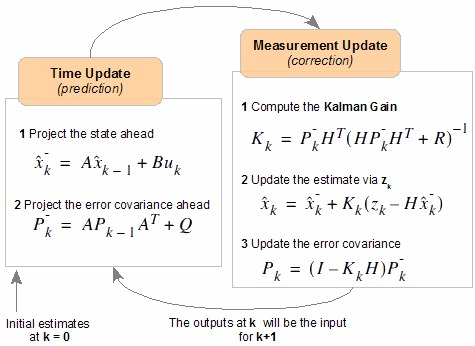
\includegraphics[scale=0.6]{images/kf_flow.jpg}
\end{figure}


\section{系统初始化(松耦合)}

在提取的图像的Features和做完IMU的预积分之后,进入了系统的初始化环节,主要的目的有以下两个:      

\begin{itemize}
\item 系统使用单目相机,如果没有一个良好的尺度估计,就无法对两个传感器做进一步的融合,这个时候需要恢复出尺度;
\item 要对IMU进行初始化,IMU会受到bias的影响,所以要得到IMU的bias。
\end{itemize}

所以我们要从初始化中恢复出尺度、重力、速度以及IMU的bias,因为视觉(SFM)在初始化的过程中有着较好的表现,所以在初始化的过程中\textbf{主要以SFM为主},然后将IMU的预积分结果与其对齐,即可得到较好的初始化结果。

\begin{itemize}
\item 根据 旋转$R$约束,估计 $\mathbf{R}_{cb}$ 和 陀螺仪Bias(加速度Bias可忽略)
\item 根据 位置$t$约束,估计 重力加速度$\mathbf{g}$ 和 尺度$s$
\item noise没法估计
\item 运动初始化
\end{itemize}

\subsection{相机与IMU之间的相对旋转(手眼标定)}

相机与IMU之间的旋转标定非常重要,\textbf{偏差1-2°系统的精度就会变的极低}\cite{xiaobuyi2018webnote}。

设相机利用对极关系得到的旋转矩阵为 $\mathbf{R}_{c_{k+1}}^{c_k}$ ,IMU经过预积分得到的旋转矩阵为 $\mathbf{R}_{b_{k+1}}^{b_{k}}$,相机与IMU之间的相对旋转为 $\mathbf{R}_{c}^{b}$,则对于任一帧满足,

\begin{equation}
\mathbf{R}^{b_{k}}_{b_{k+1}} \mathbf{R}^{b}_{c}
= \mathbf{R}^{b}_{c} \mathbf{R}^{c_{k}}_{c_{k+1}}
\end{equation}

将旋转矩阵写为四元数的形式

\begin{equation}
\mathbf{q}^{b_{k}}_{b_{k+1}} \otimes \mathbf{q}^{b}_{c}
= \mathbf{q}^{b}_{c} \otimes \mathbf{q}^{c_{k}}_{c_{k+1}}
\end{equation}

变换,写为四元数左乘矩阵和右乘矩阵的形式

\begin{equation}
({[\mathbf{q}^{b_{k}}_{b_{k+1}}]}_L - {[\mathbf{q}^{c_{k}}_{c_{k+1}}]}_R) \mathbf{q}^b_c
= \mathbf{Q}^k_{k+1} \mathbf{q}^b_c = 0
\end{equation}

$[\mathbf{q}]_L$ 与 $[\mathbf{q}]_R$ 分别表示 \textbf{四元数左乘矩阵}和\textbf{四元数右乘矩阵},其定义为(四元数实部在后)

\begin{equation}
\begin{aligned}
{[\mathbf{q}]}_L &=
{\begin{bmatrix} \mathbf{q}_v \\ q_w \end{bmatrix}}_L =
\begin{bmatrix}
{q}_{w} \mathbf{I}_{3} + {\lfloor \mathbf{q}_{v}\rfloor}_{\times} & \mathbf{q}_{v}\\
-\mathbf{q}_{v} & {q}_{w}
\end{bmatrix} \\
{[\mathbf{q}]}_R &=
{\begin{bmatrix} \mathbf{q}_v \\ q_w \end{bmatrix}}_R =
\begin{bmatrix}
{q}_{w} \mathbf{I}_{3} - {\lfloor \mathbf{q}_{v} \rfloor}_{\times} & \mathbf{q}_{v}\\
-\mathbf{q}_{v} & {q}_{w}
\end{bmatrix}
\end{aligned}
\end{equation}

那么对于 $n$对测量值,则有

\begin{equation}
\begin{bmatrix}
w^{0}_{1} \mathbf{Q}^{0}_{1} \\
w^{1}_{2} \mathbf{Q}^{1}_{2} \\
\vdots \\
w^{N-1}_{N} \mathbf{Q}^{N-1}_{N}
\end{bmatrix} 
\mathbf{q}^{b}_{c}
=
\mathbf{Q}_{N} \mathbf{q}^{b}_{c} = \boldsymbol{0}
\end{equation}

其中 $w^{k-1}_{k}$ 为外点剔除权重(Huber鲁棒核函数)

\begin{equation}
w^{k}_{k+1}
=
\left\{\begin{matrix}
1, & {\theta}^{k}_{k+1} < \text{threshold(5° as general)} \\
\frac{\text{threshold}}{\theta^{k}_{k+1}}, & \text{otherwise}
\end{matrix}\right.
\end{equation}

其与相对旋转求得的角度残差有关,$N$为计算相对旋转需要的测量对数,其由最终的终止条件决定。根据$\text{tr}(\mathbf{R}) = 1+2 \cos \theta$,角度残差可以写为

\begin{equation}
{\theta}^{k}_{k+1}
=
\arccos
\bigg(
  \frac{tr(\hat{\mathbf{R}}^{b^{-1}}_{c} \mathbf{R}^{b_{k}^{-1}}_{b_{k+1}} \hat{\mathbf{R}}^{b}_{c} \mathbf{R}^{c_{k}}_{c_{k+1}} )-1}{2}
\bigg)
\end{equation}

至此,就可以通过求解方程 $\mathbf{Q}_N \mathbf{q}_c^b = \boldsymbol{0}$ 得到相对旋转,解为 $\mathbf{Q}_N$ 的最小奇异值对应的左奇异向量。

但是,在这里还要注意 求解的终止条件(校准完成的终止条件) 。在足够多的旋转运动中,我们可以很好的估计出相对旋转 $\mathbf{R}_{c}^{b}$,这时 $\mathbf{Q}_{N}$ 对应一个准确解,且其零空间的秩为1。但是在校准的过程中,某些轴向上可能存在退化运动(如匀速运动),这时 $\mathbf{Q}_{N}$ 的零空间的秩会大于1。{\color{blue}判断条件就是 $\mathbf{Q}_N$ 的第二小的奇异值是否大于某个阈值,若大于则其零空间的秩为1,反之秩大于1,相对旋转 $\mathbf{R}_{c}^{b}$ 的精度不够,校准不成功。}  

对应代码在 \verb|InitialEXRotation::CalibrationExRotation| 中。

\begin{lstlisting}
// 相机与IMU之间的相对旋转
if(ESTIMATE_EXTRINSIC == 2)
{
    ROS_INFO("calibrating extrinsic param, rotation movement is needed");
    if (frame_count != 0)
    {
        // 选取两帧之间共有的Features
        vector<pair<Vector3d, Vector3d>> corres = f_manager.getCorresponding(frame_count - 1, frame_count);

        // 校准相机与IMU之间的旋转
        Matrix3d calib_ric;
        if (initial_ex_rotation.CalibrationExRotation(corres, pre_integrations[frame_count]->delta_q, calib_ric))
        {
            ROS_WARN("initial extrinsic rotation calib success");
            ROS_WARN_STREAM("initial extrinsic rotation: " << endl << calib_ric);
            ric[0] = calib_ric;
            RIC[0] = calib_ric;
            ESTIMATE_EXTRINSIC = 1;
        }
    }
}
\end{lstlisting}

\subsection{检测IMU可观性}

\begin{lstlisting}
// 计算均值
map<double, ImageFrame>::iterator frame_it;
Vector3d sum_g;
for (frame_it = all_image_frame.begin(), frame_it++; frame_it != all_image_frame.end(); frame_it++)
{
    double sum_dt  = frame_it->second.pre_integration->sum_dt;
    Vector3d tmp_g = frame_it->second.pre_integration->delta_v / sum_dt;
    sum_g += tmp_g;
}
Vector3d aver_g = sum_g * 1.0 / ((int)all_image_frame.size() - 1);

// 计算方差
double var = 0;
for (frame_it = all_image_frame.begin(), frame_it++; frame_it != all_image_frame.end(); frame_it++)
{
    double sum_dt  = frame_it->second.pre_integration->sum_dt;
    Vector3d tmp_g = frame_it->second.pre_integration->delta_v / sum_dt;
    var += (tmp_g - aver_g).transpose() * (tmp_g - aver_g);
}

// 计算标准差
var = sqrt(var / ((int)all_image_frame.size() - 1));
//ROS_WARN("IMU variation %f!", var);
if(var < 0.25) //! 以标准差判断可观性
{
    ROS_INFO("IMU excitation not enouth!");
    //return false;
}
\end{lstlisting}

\subsection{相机初始化(Vision-Only SFM)}

\begin{itemize}
\item 根据本质矩阵求解位姿(\verb|relativePose|)
\item 三角化特征点(\verb|sfm.construct|)
\item PnP求解位姿(\verb|cv::solvePnP|)
\item 转换到IMU坐标系下
\item $c_0$ 坐标系作为参考系
\item 不断重复直到恢复出滑窗内的Features和相机位姿
\end{itemize}

\subsection{视觉与IMU对齐}

\begin{figure}[htbp]
  \centering
  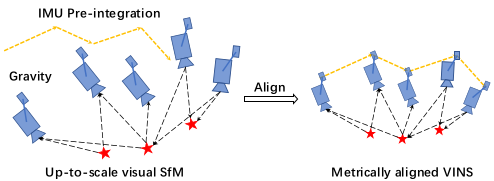
\includegraphics[scale=0.6]{images/visual_inertial_alignment.png}
\end{figure}

对应代码在\verb|VisualIMUAlignment|中,主要包括以下几个过程:
\begin{itemize}
\item Gyroscope Bias Calibration(加速度Bias相对$\mathbf{g}$非常小,不估计)
\item Velocity, Gravity Vector and Metric Scale Initialization
\item Gravity Refinement
\item Completing Initialization
\end{itemize}

\subsubsection{陀螺仪Bias标定}

该过程认为相机 $\mathbf{q}^{c_k}_{c_{k+1}}$ 较准,为真实值。

如果外参 $\mathbf{q}_{bc}$ 已经标定好,利用旋转约束,可估计陀螺仪Bias,构建最小二乘问题

\begin{equation}
{\delta \mathbf{b}_g}^{*} =
\arg \min_{\delta \mathbf{b}_g} \sum_{k\in B}
\left \| 
2 \left[
\mathbf{q}^{c_{0}^{-1}}_{b_{k+1}} \otimes \mathbf{q}^{c_{0}}_{b_{k}}
\otimes \boldsymbol{\gamma}_{b_{k+1}}^{b_{k}}
\right]_{xyz} 
\right \|^{2}
\end{equation}

其中

\begin{equation}
\boldsymbol{\gamma}_{b_{k+1}}^{b_{k}}
\approx 
\hat{\boldsymbol{\gamma}}_{b_{k+1}}^{b_{k}} \otimes 
\begin{bmatrix}
1 \\ \frac{1}{2} \mathbf{J}^{\boldsymbol{\gamma}}_{\mathbf{b}_{g}} \delta \mathbf{b}_{g}
\end{bmatrix}
\end{equation}

\begin{equation}
\mathbf{q}^{c_{0}^{-1}}_{b_{k+1}} \otimes \mathbf{q}^{c_{0}}_{b_{k}} = \mathbf{q}^{c_k}_{c_{k+1}}
\end{equation}

求取雅克比矩阵,构建正规方程$\mathbf{Hx} = \mathbf{b}$

\begin{equation}
\mathbf{J}^{\gamma^{T}}_{b_{w}} \mathbf{J}^{\gamma }_{b_{w}} \delta \mathbf{b}_{g}
=
2 \cdot \mathbf{J}^{\gamma^{T}}_{\mathbf{b}_g}
\left[
\hat{\boldsymbol{\gamma}}_{b_{k+1}}^{b_{k}^{-1}} \otimes \mathbf{q}^{c_{0}^{-1}}_{b_{k}} \otimes \mathbf{q}^{c_{0}}_{b_{k+1}}
\right]_{xyz}
\end{equation}

根据上式,即可求解 $\delta \mathbf{b}_g$,注意这个地方得到的只是Bias的变化量,需要在滑窗内累加得到Bias的准确值。   

对应代码:\verb|solveGyroscopeBias|

\begin{lstlisting}
void solveGyroscopeBias(map<double, ImageFrame> &all_image_frame, Vector3d* Bgs) {
    Matrix3d A;
    Vector3d b;
    A.setZero();
    b.setZero();

    map<double, ImageFrame>::iterator frame_i;
    map<double, ImageFrame>::iterator frame_j;
    for (frame_i = all_image_frame.begin(); next(frame_i) != all_image_frame.end(); frame_i++) {
        frame_j = next(frame_i);

        MatrixXd tmp_A(3, 3);
        VectorXd tmp_b(3);
        tmp_A.setZero();
        tmp_b.setZero();

        Eigen::Quaterniond q_ij(frame_i->second.R.transpose() * frame_j->second.R);
        tmp_A = frame_j->second.pre_integration->jacobian.template block<3, 3>(O_R, O_BG);
        tmp_b = 2 * (frame_j->second.pre_integration->delta_q.inverse() * q_ij).vec();

        A += tmp_A.transpose() * tmp_A;
        b += tmp_A.transpose() * tmp_b;
    }

    Vector3d delta_bg = A.ldlt().solve(b);
    ROS_WARN_STREAM("gyroscope bias initial calibration " << delta_bg.transpose());

    // 因为求解出的Bias是变化量,所以要累加
    for (int i = 0; i <= WINDOW_SIZE; i++)
        Bgs[i] += delta_bg;

    // 利用新的Bias重新repropagate
    for (frame_i = all_image_frame.begin(); next(frame_i) != all_image_frame.end(); frame_i++) {
        frame_j = next(frame_i);
        frame_j->second.pre_integration->repropagate(Vector3d::Zero(), Bgs[0]);
    }
}
\end{lstlisting}

\subsubsection{初始化速度、重力向量和尺度因子}

该过程要估计的状态量

\begin{equation}
\mathcal{X}_{I}=
\left[
\mathbf{v}^{b_{0}}_{b_{0}}, \mathbf{v}^{b_{0}}_{b_{1}}, \cdots, \mathbf{v}^{b_{n}}_{b_{n}}, \mathbf{g}^{c_{0}}, s
\right]
\in \mathbb{R}^{3(n+1)+3+1}
\end{equation}

其中,$\mathbf{g}^{c_{0}}$ 为在第0帧Camera相机坐标系下的重力向量。

根据IMU预积分估计模型 \eqref{equ:preinte_estimate} 可知

\begin{equation}
\begin{aligned}
\boldsymbol{\alpha}^{b_{k}}_{b_{k+1}} 
&= 
\mathbf{R}^{b_{k}}_{c_{0}}
\left(
s(\bar{\mathbf{p}}^{c_{0}}_{b_{k+1}} - \bar{\mathbf{p}}^{c_{0}}_{b_{k}}) +
\frac{1}{2}\mathbf{g}^{c_{0}} \Delta t_{k}^{2} -
\mathbf{R}^{c_0}_{b_k} \mathbf{v}^{b_k}_{b_{k}} \Delta t_{k} 
\right) 
\\
\boldsymbol{\beta}^{b_{k}}_{b_{k+1}} &=
\mathbf{R}^{b_{k}}_{c_{0}}
\left(
\mathbf{R}^{c_0}_{b_{k+1}} \mathbf{v}^{b_{k+1}}_{b_{k+1}} +
\mathbf{g}^{c_{0}}\Delta t_{k} - \mathbf{R}^{c_0}_{b_k} \mathbf{v}^{b_k}_{b_{k}}
\right)
\end{aligned}
\end{equation}

我们已经得到了IMU相对于相机的旋转 $\mathbf{q}_{b}^{c}$,假设IMU到相机的平移量$\mathbf{p}_{b}^{c}$,那么可以很容易地将相机坐标系下的位姿转换到IMU坐标系下。

\begin{equation}
\begin{aligned}
\mathbf{q}_{b_{k}}^{c_{0}} &=
\mathbf{q}^{c_{0}}_{c_{k}} \otimes (\mathbf{q}_{c}^{b})^{-1}  \\
s \bar{\mathbf{p}}^{c_{0}}_{b_{k}} &=
s \bar{\mathbf{p}}^{c_{0}}_{c_{k}} - \mathbf{R}^{c_{0}}_{b_{k}} \mathbf{p}_{c}^{b}
\end{aligned}
\end{equation}

所以,定义相邻两帧之间的IMU预积分测量值(${\hat{\boldsymbol{\alpha}}}_{b_{k+1}}^{b_{k}}$,${\hat{\boldsymbol{\beta}}}_{b_{k+1}}^{b_{k}}$)与预积分估计值之间的残差,即

\begin{equation}
\begin{aligned}
\mathbf{r}(\hat{\mathbf{z}}^{b_{k}}_{b_{k+1}}, \mathcal{X}_I) 
&=
\begin{bmatrix}
\delta \boldsymbol{\alpha}^{b_{k}}_{b_{k+1}} \\
\delta \boldsymbol{\beta}^{b_{k}}_{b_{k+1}}
\end{bmatrix} \\ 
&=
\begin{bmatrix}
\hat{\boldsymbol{\alpha}}^{b_{k}}_{b_{k+1}} -& 
\mathbf{R}^{b_{k}}_{c_{0}}
\left(
s(\bar{\mathbf{p}}^{c_{0}}_{b_{k+1}} - \bar{\mathbf{p}}^{c_{0}}_{b_{k}}) +
\frac{1}{2}\mathbf{g}^{c_{0}} \Delta t_{k}^{2} -
\mathbf{R}^{c_0}_{b_k} \mathbf{v}^{b_k}_{b_{k}} \Delta t_{k} 
\right) \\
\hat{\boldsymbol{\beta}}^{b_{k}}_{b_{k+1}} -&
\mathbf{R}^{b_{k}}_{c_{0}}
\left(
\mathbf{R}^{c_0}_{b_{k+1}} \mathbf{v}^{b_{k+1}}_{b_{k+1}} +
\mathbf{g}^{c_{0}}\Delta t_{k} - \mathbf{R}^{c_0}_{b_k} \mathbf{v}^{b_k}_{b_{k}}
\right)
\end{bmatrix}
\end{aligned}
\end{equation}

令 $\mathbf{r}(\hat{z}_{b_{k+1}}^{b_{k}}, \mathcal{X}_I)=\mathbf{0}$,转换成 $\mathbf{Hx}=\mathbf{b}$ 的形式

\begin{equation}
\label{equ:init_vgs}
\begin{bmatrix}
-\mathbf{I} \Delta t_{k} & 0 & \frac{1}{2} \mathbf{R}^{b_{k}}_{c_{0}} \Delta t_{k}^{2} &
\mathbf{R}^{b_{k}}_{c_{0}} (\bar{\mathbf{p}}^{c_{0}}_{c_{k+1}} - \bar{\mathbf{p}}^{c_{0}}_{c_{k}}) \\
-\mathbf{I} & \mathbf{R}^{b_{k}}_{c_{0}} \mathbf{R}^{c_0}_{b_{k+1}} & \mathbf{R}^{b_{k}}_{c_{0}}\Delta t_{k} & 0
\end{bmatrix}
\begin{bmatrix}
\mathbf{v}^{b_{k}}_{b_{k}}\\
\mathbf{v}^{b_{k+1}}_{b_{k+1}}\\
\mathbf{g}^{c_{0}}\\
s
\end{bmatrix} 
=
\begin{bmatrix}
\boldsymbol{\alpha}^{b_{k}}_{b_{k+1}} - \mathbf{p}_c^b + \mathbf{R}^{b_{k}}_{c_{0}} \mathbf{R}^{c_0}_{b_{k+1}} \mathbf{p}_c^b \\
\boldsymbol{\beta}^{b_{k}}_{b_{k+1}}
\end{bmatrix}
\end{equation}

通过Cholosky分解求解 $\mathcal{X}_I$

\begin{equation}
\mathbf{H}^T \mathbf{H} \mathcal{X}_I = \mathbf{H}^T \mathbf{b}
\end{equation}

对应代码在 \verb|LinearAlignment|。

\subsubsection{优化重力}

\begin{figure}[htbp]
\centering
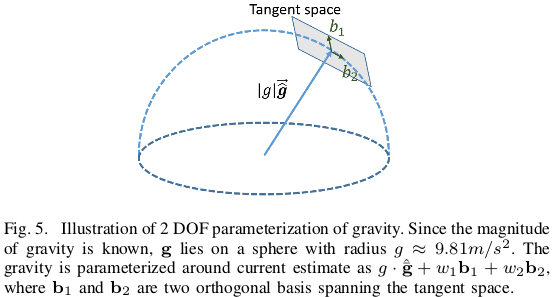
\includegraphics[scale=0.6]{images/gravity_tangent_space.png}
\end{figure}

利用公式\eqref{equ:init_vgs}求解重力向量$\mathbf{g}^{c_0}$的过程中,并没有加入模长限制$\|\mathbf{g}^{c_0}\|=9.81$。三维变量$\mathbf{g}^{c_0}$实际只有2个自由度。

重力矢量有2个自由度,在切空间上对其参数化:

\begin{equation}
\begin{aligned}
\hat{\mathbf{g}}^{c_0}
&=
\|\mathbf{g}\| \cdot \bar{\hat{\mathbf{g}}}^{c_0} + \omega_1 \vec{b_1} + \omega_2 \vec{b_2} \\ 
&=
\|\mathbf{g}\| \cdot \bar{\hat{\mathbf{g}}}^{c_0} + \mathbf{B} \vec{\omega}
\end{aligned} , \quad
\mathbf{B} 
=
\begin{bmatrix}
\vec{b_1} & \vec{b_2}
\end{bmatrix} 
\in \mathbb{R}^{3 \times 2}, \vec{\omega} \in \mathbb{R}^{2 \times 1}
\end{equation}

其中,$\omega_1$、$\omega_2$为待优化变量,$\vec{b}_{1}$、$\vec{b}_{1}$分别为

\begin{equation}
\begin{array}{l}{
\vec{b}_{1} =
\left\{\begin{array}{ll}
{\left(\hat{\mathbf{g}}^{c_{0}} \times [1,0,0] \right),} & 
{\hat{\mathbf{g}}^{c_{0}} \neq[1,0,0]^{\top}} \\ 
{\left(\hat{\mathbf{g}}^{c_{0}} \times [0,0,1] \right),} & {\text{otherwise}}
\end{array}\right.} 
\\ 
{\vec{b}_{2}=\hat{\overline{\mathbf{g}}}^{c_{0}} \times \vec{b}_{1}}
\end{array}
\end{equation}

将$\mathbf{g}^{c_0}$代入上一小节公式\eqref{equ:init_vgs}得

\begin{equation}
\begin{aligned}
\begin{bmatrix}
-\mathbf{I} \Delta t_{k} & 0 & \frac{1}{2} \mathbf{R}^{b_{k}}_{c_{0}} \Delta t_{k}^{2} \mathbf{B} &
\mathbf{R}^{b_{k}}_{c_{0}} (\bar{\mathbf{p}}^{c_{0}}_{c_{k+1}} - \bar{\mathbf{p}}^{c_{0}}_{c_{k}}) \\
-\mathbf{I} & \mathbf{R}^{b_{k}}_{c_{0}} \mathbf{R}^{c_0}_{b_{k+1}} & \mathbf{R}^{b_{k}}_{c_{0}}\Delta t_{k} \mathbf{B} & 0
\end{bmatrix}
\begin{bmatrix}
\mathbf{v}^{b_{k}}_{b_{k}} \\
\mathbf{v}^{b_{k+1}}_{b_{k+1}} \\
\vec{\omega} \\
s
\end{bmatrix} 
\\=
\begin{bmatrix}
\boldsymbol{\alpha}^{b_{k}}_{b_{k+1}} - \mathbf{p}_c^b + \mathbf{R}^{b_{k}}_{c_{0}} \mathbf{R}^{c_0}_{b_{k+1}} \mathbf{p}_c^b -
\frac{1}{2} \mathbf{R}^{b_{k}}_{c_{0}} \Delta t_{k}^{2} \|\mathbf{g}\| \cdot \bar{\hat{\mathbf{g}}}\\
\boldsymbol{\beta}^{b_{k}}_{b_{k+1}} -
\mathbf{R}^{b_{k}}_{c_{0}} \Delta t_{k} \|\mathbf{g}\| \cdot \bar{\hat{\mathbf{g}}}
\end{bmatrix}
\end{aligned}
\end{equation}

同样,通过Cholosky分解求得 $\vec{\omega}$,得到 相机$C_0$系下的重力向量$\hat{\mathbf{g}}^{c_0}$。

对应代码在\verb|RefineGravity|中。

\subsubsection{将相机坐标系对齐到世界坐标系}

通过将 $\mathbf{g}^{c_{0}}$ 旋转至惯性坐标系(世界系)中的 z 轴方向[0,0,1],可以计算第一帧相机系到惯性系的旋转矩阵 $\mathbf{q}_{c_0}^w$,这样就可以将所有变量调整至惯性世界系(\textbf{水平坐标系},z轴与重力方向对齐)中。

找到$c_0$到$w$系的旋转矩阵$\mathbf{R}_{w c_{0}}=\exp ([\theta \mathbf{u}])$

\begin{equation}
\mathbf{u}
=
\frac{\hat{\mathbf{g}}^{c_{0}} \times \hat{\mathbf{g}}^{w}}{\left\|\hat{\mathbf{g}}^{c_{0}} \times \hat{\mathbf{g}}^{w}\right\|}, \quad 
\theta
=
\operatorname{atan} 2\left(\left\|\hat{\mathbf{g}}^{c_{0}} \times \hat{\mathbf{g}}^{w}\right\|, \hat{\mathbf{g}}^{c_{0}} \cdot \hat{\mathbf{g}}^{w}\right)
\end{equation}

把所有$c_0$坐标系下的变量旋转到$w$下,把相机平移和特征点尺度恢复到米制单位,完成了系统初始化过程。


\section{后端优化(紧耦合)}

\begin{figure}[htbp]
\centering
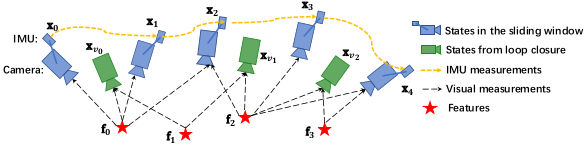
\includegraphics[scale=0.6]{images/sliding_window_vio.png}
\end{figure}

VIO 紧耦合方案的主要思路就是通过将基于视觉构造的残差项和基于IMU构造的残差项放在一起构造成一个联合优化的问题,整个优化问题的最优解即可认为是比较准确的状态估计。

为了限制优化变量的数目,VINS-Mono 采用了滑动窗口的形式,\textbf{滑动窗口中的全状态量}:

\begin{equation}
\begin{aligned}
\mathcal{X} 
&= 
\left[
\mathbf{x}_{0},\mathbf{x}_{1},\cdots,\mathbf{x}_{n},\mathbf{x}^{b}_{c},{\lambda}_{0},{\lambda}_{1}, \cdots ,{\lambda}_{m}
\right]  
\\
\mathbf{x}_{k} 
&= 
\left[
\mathbf{p}^{w}_{b_{k}},\mathbf{v}^{w}_{b_{k}},\mathbf{q}^{w}_{b_{k}},\mathbf{b}_{a},\mathbf{b}_{g}
\right], \quad k \in [0,n] 
\\
\mathbf{x}^{b}_{c} &= \left[ \mathbf{p}^{b}_{c}, \mathbf{q}^{b}_{c} \right]
\end{aligned}
\end{equation}

\begin{itemize}
\item 滑动窗口内 n+1 个所有相机的状态(包括位置、朝向、速度、加速度计 bias 和陀螺仪 bias)
\item Camera 到 IMU 的外参
\item m+1 个 3D 点的逆深度
\end{itemize}

优化过程中的 \textbf{误差状态量}

\begin{equation}
\begin{aligned}
\delta \mathcal{X}
&=
\left[
\delta \mathbf{x}_{0}, \delta \mathbf{x}_{1}, \cdots, \delta \mathbf{x}_{n}, \delta \mathbf{x}^{b}_{c}, \lambda_{0}, \delta \lambda_{1}, \cdots, \delta \lambda_{m}
\right] 
\\
\delta \mathbf{x}_{k}
&=
\left[
\delta \mathbf{p}^{w}_{b_{k}}, \delta \mathbf{v}^{w}_{b_{k}}, \delta \boldsymbol{\theta}^{w}_{b_{k}}, \delta \mathbf{b}_{a}, \delta \mathbf{b}_{g}
\right], \quad k \in [0,n] \\
\delta \mathbf{x}^{b}_{c} &= \left[ \delta \mathbf{p}^{b}_{c}, \delta \mathbf{q}^{b}_{c} \right] 
\end{aligned}
\end{equation}

进而得到系统优化的代价函数(Minimize residuals from all sensors)

\begin{equation}
\min_{\mathcal{X}}
\left\{
\underbrace{
\left\|\mathbf{r}_{p}-\mathbf{H}_{p} \mathcal{X}\right\|^{2}
}_\text{边缘化先验}
+
\underbrace{
\sum_{k \in \mathcal{B}}\left\|\mathbf{r}_{\mathcal{B}}\left(\hat{\mathbf{z}}_{b_{k+1}}^{b_{k}}, \mathcal{X}\right)\right\|_{\mathbf{P}_{b_{k}+1}^{2}}^{2}
}_\text{IMU残差}
+
\underbrace{
\sum_{(l, j) \in \mathcal{C}} \rho\left(\left\|\mathbf{r}_{\mathcal{C}}\left(\hat{\mathbf{z}}_{l}^{c_{j}}, \mathcal{X}\right)\right\|_{\mathbf{P}_{l}^{c_{j}}}^{2}\right)
}_\text{视觉残差}
\right\}
\end{equation}

其中,
\begin{itemize}
\item 三个残差都是用 \textbf{马氏距离}(与量纲无关)来表示的
\item 鲁邦核函数 $\rho(\cdot)$ 仅处理视觉outlier
\end{itemize}

\textbf{Motion-only visual-inertial bundle adjustment}: Optimize \textbf{position, velocity, rotation} in a smaller windows, assuming all other quantities are fixed

\subsection{IMU 测量残差}

\begin{enumerate}

\item IMU 测量残差

根据上面的IMU预积分,得到 \textbf{IMU预积分残差}(\textbf{估计值 - 测量值})

\begin{equation}
\label{equ:residual_imu_origin}
\mathbf{r}_{\mathcal{B}}\left(\hat{\mathbf{z}}_{b_{k+1}}^{b_{k}}, \mathcal{X}\right) 
=
\left[\begin{array}{c}
{\delta \boldsymbol{\alpha}_{b_{k+1}}^{b_{k}}} \\ 
{\delta \boldsymbol{\theta}_{b_{k+1}}^{b_{k}}} \\
{\delta \boldsymbol{\beta}_{b_{k+1}}^{b_{k}}} \\ 
{\delta \mathbf{b}_{b_{k}}} \\ 
{\delta \mathbf{b}_{g_{k}}}
\end{array}\right]_{15 \times 1} 
= 
\left[\begin{array}{c}
{\mathbf{R}_{w}^{b_{k}}
\left(\mathbf{p}_{b_{k+1}}^{w}-\mathbf{p}_{b_{k}}^{w}+\frac{1}{2} \mathbf{g}^{w} \Delta t_{k}^{2}-\mathbf{v}_{b_{k}}^{w} \Delta t_{k}\right)-
\color{blue}{\boldsymbol{\alpha}_{b_{k+1}}^{b_{k}}}} \\ 
{2\left[\mathbf{q}_{b_{k}}^{w^{-1}} \otimes \mathbf{q}_{b_{k+1}}^{w} \otimes\left({\color{blue}{{\gamma}_{b_{k+1}}^{b_{k}}}}\right)^{-1}\right]_{x y z}} \\
{\mathbf{R}_{w}^{b_{k}}\left(\mathbf{v}_{b_{k+1}}^{w}+\mathbf{g}^{w} \Delta t_{k}-\mathbf{v}_{b_{k}}^{w}\right) - \color{blue}{\boldsymbol{\beta}}_{b_{k+1}}^{b_{k}}} \\  
{\mathbf{b}_{a b_{k+1}}-\mathbf{b}_{a b_{k}}} \\ 
{\mathbf{b}_{w b_{k+1}}-\mathbf{b}_{w b_{k}}}
\end{array}\right]
\end{equation}

其中 $[\color{blue}{{\alpha}^{b_{k}}_{b_{k+1}},{\gamma}^{b_{k}}_{b_{k+1}},{\beta}^{b_{k}}_{b_{k+1}}}]$ 为 \textbf{IMU预积分测量Bias修正值}。

将式\eqref{equ:residual_imu_origin} 写成四元数形式

\begin{equation}
\label{equ:residual_imu_q}
\mathbf{r}_{\mathcal{B}}
=
\left[\begin{array}{c}
{\mathbf{r}_{p}} \\ 
{\mathbf{r}_{q}} \\ 
{\mathbf{r}_{v}} \\ 
{\mathbf{r}_{b a}} \\ 
{\mathbf{r}_{b g}}
\end{array}\right]
=
\left[\begin{array}{c}
{\mathbf{q}_{b_{i} w}\left(\mathbf{p}_{w b_{j}}-\mathbf{p}_{w b_{i}}-\mathbf{v}_{i}^{w} \Delta t+\frac{1}{2} \mathbf{g}^{w} \Delta t^{2}\right)-{\color{blue}\boldsymbol{\alpha}_{b_{i} b_{j}}}} \\ 
{2\left[{\color{blue}\mathbf{q}_{b_{j} b_{i}}} \otimes\left(\mathbf{q}_{b_{i} w} \otimes \mathbf{q}_{w b_{j}}\right)\right]_{xyz}} \\ 
{\mathbf{q}_{b_{i} w}\left(\mathbf{v}_{j}^{w}-\mathbf{v}_{i}^{w}+\mathbf{g}^{w} \Delta t\right)-{\color{blue}\boldsymbol{\beta}_{b_{i} b_{j}}}} \\ 
{\mathbf{b}_{j}^{a}-\mathbf{b}_{i}^{a}} \\ 
{\mathbf{b}_{j}^{g}-\mathbf{b}_{i}^{g}}
\end{array}\right]_{15 \times 1}
\end{equation}

\begin{lstlisting}
Eigen::Quaterniond dq_rected = delta_q * Utility::deltaQ(dq_dbg * dbg);
Eigen::Vector3d    dv_rected = delta_v + dv_dba * dba + dv_dbg * dbg;
Eigen::Vector3d    dp_rected = delta_p + dp_dba * dba + dp_dbg * dbg;

residuals.block<3, 1>(O_P, 0)  = 
    Qi.inverse() * (0.5*G*sum_dt*sum_dt + Pj - Pi - Vi*sum_dt) - dp_rected;
residuals.block<3, 1>(O_R, 0)  = 
    2 * (dq_rected.inverse() * (Qi.inverse() * Qj)).vec();
residuals.block<3, 1>(O_V, 0)  = 
    Qi.inverse() * (G * sum_dt + Vj - Vi) - dv_rected;
residuals.block<3, 1>(O_BA, 0) = Baj - Bai;
residuals.block<3, 1>(O_BG, 0) = Bgj - Bgi;
\end{lstlisting}

\item 协方差矩阵

此处用到的协方差矩阵为前面IMU预积分计算出的协方差矩阵 $\mathbf{P}$。

残差的后处理对应代码:

\begin{lstlisting}
Eigen::Map<Eigen::Matrix<double, 15, 1>> residual(residuals);
residual=pre_integration->evaluate(Pi, Qi, Vi, Bai, Bgi, Pj, Qj, Vj, Baj, Bgj);

Eigen::Matrix<double, 15, 15> cov_inv = pre_integration->covariance.inverse();
Eigen::Matrix<double, 15, 15> sqrt_info =
    Eigen::LLT<Eigen::Matrix<double, 15, 15>>(cov_inv).matrixL().transpose();

residual = sqrt_info * residual; 
\end{lstlisting}

这里残差 \verb|residual| 乘以 \verb|sqrt_info|,是因为真正的优化项其实是 Mahalanobis 距离 或 马氏范数

\begin{equation}
\|\mathbf{r}\|^2_{\boldsymbol{\Sigma}} = \mathbf{r}^T \boldsymbol{\Sigma}^{-1} \mathbf{r}
\end{equation}

Mahalanobis距离 其实相当于一个残差加权,协方差大的加权小,协方差小的加权大,着重优化那些比较确定的残差。  

Ceres-Solver只接受最小二乘优化,即 $\min \|\mathbf{r}\|^2$,通过Cholesky分解,\textbf{将马氏范数转化为二范数}

\begin{equation}
\|\mathbf{r}\|^2_{\boldsymbol{\Sigma}} 
= 
\mathbf{r}^T \boldsymbol{\Sigma}^{-1} \mathbf{r}
=
\mathbf{r}^T (\mathbf{L} \mathbf{L}^T) \mathbf{r}
=
(\mathbf{L}^T \mathbf{r})^T (\mathbf{L}^T \mathbf{r})
=
\|\mathbf{L}^T \mathbf{r}\|^2
\end{equation}

令 $\mathbf{r'} = (\mathbf{L}^T \mathbf{r})$ 作为新的优化误差,所以 

\begin{equation}
\text{sqrt\_info} = \mathbf{L}^T
\end{equation}

\item 雅克比矩阵

高斯迭代优化过程中会用到IMU测量残差对状态量的雅克比矩阵,但此处我们是 \textbf{对误差状态量求偏导},下面根据式\eqref{equ:residual_imu_q} 对四部分误差状态量求取雅克比矩阵。

\begin{enumerate}

\item 对 {\color{blue}i 时刻 $[\delta p^{w}_{b_{i}},\delta \theta ^{w}_{b_{i}}]$} 求偏导

\begin{equation}
\mathbf{J}[0]=
\begin{bmatrix}
-\mathbf{R}_{b_{i} w} & \left[\mathbf{R}_{b_{i} w}\left(\mathbf{p}_{w b_{j}}-\mathbf{p}_{w b_{i}}-\mathbf{v}_{i}^{w} \Delta t+\frac{1}{2} \mathbf{g}^{w} \Delta t^{2}\right)\right]_{\times} \\
\mathbf{0} & -2\left[\begin{array}{ll}{\mathbf{0}} & {\mathbf{I}}\end{array}\right]\left[\mathbf{q}_{w b_{j}}^{*} \otimes \mathbf{q}_{w b_{i}}\right]_{L}\left[\mathbf{q}_{b_{i} b_{j}}\right]_{R}\left[\begin{array}{c}{\mathbf{0}} \\ {\frac{1}{2} \mathbf{I}}\end{array}\right] \\
\mathbf{0} & \left[\mathbf{R}_{b_{i} w}\left(\mathbf{v}_{j}^{w}-\mathbf{v}_{i}^{w}+\mathbf{g}^{w} \Delta t\right)\right]_{\times} \\
\mathbf{0} & \mathbf{0}  \\
\mathbf{0} & \mathbf{0} 
\end{bmatrix}
\in \mathbb{R}^{15 \times 7}
\end{equation}

\item 对 {\color{blue}i 时刻 $[\delta v^{w}_{i},\delta b^a_{i},\delta b^g_{i}]$} 求偏导

\begin{equation}
\mathbf{J}[1]=
\begin{bmatrix}
-\mathbf{R}_{b_{i} w} \Delta t & -\mathbf{J}_{b_{i}^{a}}^{\alpha} & -\mathbf{J}_{b_{i}^{g}}^{\alpha} \\
\mathbf{0} & \mathbf{0} & -2\left[\begin{array}{ll}{\mathbf{0}} & {\mathbf{I}}\end{array}\right]\left[\mathbf{q}_{w b_{j}}^{*} \otimes \mathbf{q}_{w b_{i}} \otimes \mathbf{q}_{b_{i} b_{j}}\right]_{L}\left[\begin{array}{c}{\mathbf{0}} \\ {\frac{1}{2} \mathbf{J}_{b_{i}^{g}}^{q}}\end{array}\right] \\
-\mathbf{R}_{b_{i} w} & -\mathbf{J}_{b_{i}^{a}}^{\beta} & -\mathbf{J}_{b_{i}^{g}}^{\beta} \\
\mathbf{0} & -\mathbf{I}  &  \mathbf{0} \\
\mathbf{0} &  \mathbf{0}  & -\mathbf{I}
\end{bmatrix}
\in \mathbb{R}^{15 \times 9}
\end{equation}

\item 对 {\color{blue}j 时刻 $[\delta p^{w}_{b_{j}},\delta \theta ^{w}_{b_{j}}]$} 求偏导

\begin{equation}
\mathbf{J}[2]=
\begin{bmatrix}
\mathbf{R}_{b_{i} w} & \mathbf{0} \\
\mathbf{0} & 2\left[\begin{array}{ll}{\mathbf{0}} & {\mathbf{I}}\end{array}\right]\left[\mathbf{q}_{b_{i} b_{j}}^{*} \otimes \mathbf{q}_{w b_{i}}^{*} \otimes \mathbf{q}_{w b_{j}}\right]_{L}\left[\begin{array}{c}{\mathbf{0}} \\ {\frac{1}{2} \mathbf{I}}\end{array}\right] \\
\mathbf{0} & \mathbf{0} \\
\mathbf{0} & \mathbf{0}  \\
\mathbf{0} & \mathbf{0}   
\end{bmatrix}
\in \mathbb{R}^{15 \times 7}
\end{equation}

\item 对 {\color{blue}j 时刻 $[\delta v^{w}_{j},\delta b^a_{j},\delta b^g_{j}]$} 求偏导

\begin{equation}
\mathbf{J}[3]=
\begin{bmatrix}
\mathbf{0} & \mathbf{0} & \mathbf{0} \\
\mathbf{0} & \mathbf{0} & \mathbf{0} \\
\mathbf{R}_{b_{i} w} & \mathbf{0} & \mathbf{0} \\
\mathbf{0} & \mathbf{I} & \mathbf{0} \\
\mathbf{0} & \mathbf{0} & \mathbf{I}
\end{bmatrix}
\in \mathbb{R}^{15 \times 9}
\end{equation}

\end{enumerate}

雅克比矩阵计算的对应代码在\verb|class IMUFactor : public ceres::SizedCostFunction| 中的 \verb|Evaluate()| 函数中。

\end{enumerate}

\subsection{视觉测量残差}

视觉测量残差 即 \textbf{特征点的重投影误差},视觉残差和雅克比矩阵计算的对应代码在\verb|ProjectionFactor::Evaluate| 函数中。

\begin{enumerate}

\item 重投影误差(视觉测量残差)

对于第 i 帧中的特征点,它投影到第 j 帧相机坐标系下的值为

\begin{equation}
\left[\begin{array}{c}
{x_{c_{j}}} \\ {y_{c_{j}}} \\ {z_{c_{j}}} \\ {1}
\end{array}\right] =
\mathbf{T}_{b c}^{-1} 
\mathbf{T}_{w b_{j}}^{-1} 
\mathbf{T}_{w b_{i}} 
\mathbf{T}_{b c}
\left[\begin{array}{c}
{\frac{1}{\lambda} u_{c_{i}}} \\ 
{\frac{1}{\lambda} v_{c_{i}}} \\ 
{\frac{1}{\lambda}} \\ 
{1}
\end{array}\right]
\end{equation}

拆成三维坐标形式为

\begin{equation}
\label{equ:pcj}
\begin{aligned} 
\mathbf{P}_{c_{j}} 
&=
\left[\begin{array}{c}
{x_{c_{j}}} \\ {y_{c_{j}}} \\ {z_{c_{j}}}
\end{array}\right] 
=
\mathbf{R}_{b c}^{\top} \left(
\mathbf{R}_{w b_{j}}^{\top} \left(
\mathbf{R}_{w b_{i}} \left(
\mathbf{R}_{b c} 
\mathbf{P}_{c_i}
+ \mathbf{p}_{b c} \right)
+ \mathbf{p}_{w b_{i}} - \mathbf{p}_{w b_{j}}\right)
- \mathbf{p}_{b c}\right) \\
&=
\mathbf{R}_{b c}^{\top} 
\mathbf{R}_{w b_{j}}^{\top} 
\mathbf{R}_{w b_{i}} 
\mathbf{R}_{b c} 
\mathbf{P}_{c_i} +
\mathbf{R}_{b c}^{\top}
\left(\mathbf{R}_{w b_{j}}^{\top} 
\left(\left(\mathbf{R}_{w b_{i}} \mathbf{p}_{b c}+\mathbf{p}_{w b_{i}}\right)
-\mathbf{p}_{w b_{j}}\right)-\mathbf{p}_{b c}\right) 
\end{aligned}
\end{equation}

其中,

\begin{equation}
\label{equ:pci}
\mathbf{P}_{c_i} = \frac{\bar{\mathbf{P}}_{c_{i}}}{\lambda} = 
\frac{1}{\lambda}
\left[\begin{array}{c}
{u_{c_{i}}} \\ {v_{c_{i}}} \\ {1}
\end{array}\right]
\end{equation}

为了后面方便求Jacobian,对式\eqref{equ:pcj}拆解,定义如下变量

\begin{equation}
\label{equ:f_predef}
\begin{array}{l}
{\mathbf{f}_{b_{i}}=\mathbf{R}_{b c} \mathbf{P}_{c_{i}}+\mathbf{p}_{b c}} \\ {\mathbf{f}_{w}=\mathbf{R}_{w b_{i}} \mathbf{f}_{b_{i}}+\mathbf{p}_{w b_{i}}} \\ {\mathbf{f}_{b_{j}}=\mathbf{R}_{w b_{j}}^{\top}\left(\mathbf{f}_{w}-\mathbf{p}_{w b_{j}}\right)} \\
{\mathbf{P}_{c_{j}}=\mathbf{R}_{b c}^{\top}\left(\mathbf{f}_{b_{j}}-\mathbf{p}_{b c}\right)}
\end{array}
\end{equation}

\begin{lstlisting}
// 将第i frame下的3D点转到第j frame坐标系下
Eigen::Vector3d pts_camera_i = pts_i / inv_dep_i;
Eigen::Vector3d pts_imu_i    = qic * pts_camera_i + tic;
Eigen::Vector3d pts_w        = Qi * pts_imu_i + Pi;     
Eigen::Vector3d pts_imu_j    = Qj.inverse() * (pts_w - Pj); 
Eigen::Vector3d pts_camera_j = qic.inverse() * (pts_imu_j - tic);
\end{lstlisting}

视觉测量残差为

\begin{equation}
\label{equ:residual_visual}
\mathbf{r}_{c} =
\Sigma \cdot
\left[\begin{array}{c}
{\frac{x_{c_{j}}}{z_{c_{j}}}-u_{c_{j}}} \\ 
{\frac{y_{c_{j}}}{z_{c_{j}}}-v_{c_{j}}}
\end{array}\right] =
\Sigma \cdot
\left(\frac{P_{c_{j}}}{Z_j} - \hat{\bar{P}}_{c_{j}}\right)_2
\in \mathbb{R}^{2 \times 1}
\end{equation}

\begin{lstlisting}
Eigen::Map<Eigen::Vector2d> residual(residuals);
#ifdef UNIT_SPHERE_ERROR
// why
// 把归一化平面上的重投影误差投影到Unit sphere上的好处就是可以支持所有类型的相机
// 求取切平面上的误差
residual =  tangent_base * (pts_camera_j.normalized() - pts_j.normalized());
#else
// 求取归一化平面上的误差
double dep_j = pts_camera_j.z();
residual = (pts_camera_j / dep_j).head<2>() - pts_j.head<2>();
#endif
residual = sqrt_info * residual; // 转成与量纲无关的马氏距离
\end{lstlisting}

\item 协方差矩阵

固定的协方差矩阵,归一化平面的标准差为 $\frac{1.5}{f}$,即像素标准差为 $1.5$

\begin{equation}
\Sigma = 
\begin{bmatrix}
\frac{f}{1.5} & 0 \\
0 & \frac{f}{1.5}
\end{bmatrix}
\end{equation}

\begin{lstlisting}
ProjectionFactor::sqrt_info = FOCAL_LENGTH / 1.5 * Matrix2d::Identity();
\end{lstlisting}

\item 雅克比矩阵

Jacobian 为视觉误差对两个时刻的状态量、外参以及逆深度求导

\begin{equation}
\mathbf{J} = 
\frac{\partial \mathbf{r}_{c}}{\partial \mathbf{X}_{c}} =
\begin{bmatrix}
\frac{\partial \mathbf{P}_{c_{j}}}
{\partial\left[\begin{array}{c}{\delta \mathbf{p}_{w b_{i}}} \\ 
{\delta \boldsymbol{\theta}_{w b_{i}}}\end{array}\right]} 
&
\frac{\partial \mathbf{P}_{c_{j}}}
{\partial\left[\begin{array}{c}{\delta \mathbf{p}_{w b_{j}}} \\ 
{\delta \boldsymbol{\theta}_{w b_{j}}}\end{array}\right]} 
&
\frac{\partial \mathbf{P}_{c_{j}}}
{\partial\left[\begin{array}{c}{\delta \mathbf{p}_{bc}} \\ 
{\delta \boldsymbol{\theta}_{bc}}\end{array}\right]} 
&
\frac{\partial \mathbf{P}_{c_{j}}}{\partial \delta \lambda}
\end{bmatrix}
\end{equation}

根据链式法则

\begin{equation}
\begin{aligned}
\mathbf{J} 
&= 
\frac{\partial \mathbf{r}_{c}}{\partial \mathbf{P}_{c_{j}}}
\frac{\partial \mathbf{P}_{c_{j}}}{\partial \mathbf{X}_{c}}
=
\mathbf{J}_1 \mathbf{J}_2 \\
&=
\frac{\partial \mathbf{r}_{c}}{\partial \mathbf{P}_{c_{j}}}
\begin{bmatrix}
\frac{\partial \mathbf{P}_{c_{j}}}
{\partial\left[\begin{array}{c}{\delta \mathbf{p}_{w b_{i}}} \\ 
{\delta \boldsymbol{\theta}_{w b_{i}}}\end{array}\right]} 
&
\frac{\partial \mathbf{P}_{c_{j}}}
{\partial\left[\begin{array}{c}{\delta \mathbf{p}_{w b_{j}}} \\ 
{\delta \boldsymbol{\theta}_{w b_{j}}}\end{array}\right]} 
&
\frac{\partial \mathbf{P}_{c_{j}}}
{\partial\left[\begin{array}{c}{\delta \mathbf{p}_{bc}} \\ 
{\delta \boldsymbol{\theta}_{bc}}\end{array}\right]} 
&
\frac{\partial \mathbf{P}_{c_{j}}}{\partial \delta \lambda}
\end{bmatrix}
\end{aligned}
\end{equation}

先求$\mathbf{J}$的第一部分 $\mathbf{J}_1$,根据式\eqref{equ:residual_visual}

\begin{equation}
\mathbf{J}_1 =
\frac{\partial \mathbf{r}_{c}}{\partial \mathbf{P}_{c_{j}}} = 
\Sigma \cdot
\left[\begin{array}{ccc}
{\frac{1}{z_{c_{j}}}} & {0} & {-\frac{x_{c_{j}}}{z_{c_{j}}^{2}}} \\ 
{0} & {\frac{1}{z_{c_{j}}}} & {-\frac{y_{c_{j}}^{2}}{z_{c_{j}}^{2}}}
\end{array}\right]
\in \mathbb{R}^{2 \times 3}
\end{equation}

\begin{lstlisting}
Eigen::Matrix<double, 2, 3> reduce(2, 3);
reduce << 1. / dep_j, 0, -pts_camera_j(0) / (dep_j * dep_j),
          0, 1. / dep_j, -pts_camera_j(1) / (dep_j * dep_j);
reduce = sqrt_info * reduce;
\end{lstlisting}

再求$\mathbf{J}$的第二部分 $\mathbf{J}_2$,根据式\eqref{equ:pcj}\eqref{equ:pci}\eqref{equ:f_predef},对各状态量求偏导。

\begin{enumerate}

\item 对 {\color{blue} $i$ 时刻的状态量 $[\delta p^{w}_{b_{i}},\delta \theta ^{w}_{b_{i}}]$} 求偏导

\begin{equation}
\begin{aligned}
\frac{\partial \mathbf{P}_{c_{j}}}{\partial \delta \mathbf{p}_{w b_{i}}} 
&=
\mathbf{R}_{b c}^{\top} \mathbf{R}_{w b_{j}}^{\top} 
\\
\frac{\partial \mathbf{P}_{c_{j}}}{\partial \delta \boldsymbol{\theta}_{w b_{i}}} 
&=
\frac{\partial \mathbf{R}_{b c}^{\top} \mathbf{R}_{w b_{j}}^{\top} \mathbf{R}_{w b_{i}}\left(\mathbf{I}+\left[\delta \boldsymbol{\theta}_{wb_{i}}\right]_{\times}\right) \mathbf{f}_{b_{i}}}{\partial \delta \boldsymbol{\theta}_{wb_{i}}} 
\quad \text{(丢弃了不相关部分)} \\
&=
-\mathbf{R}_{b c}^{\top} \mathbf{R}_{w b_{j}}^{\top} \mathbf{R}_{w b_{i}}\left[\mathbf{f}_{b_{i}}\right]_{\times}
\end{aligned}
\end{equation}

\begin{equation}
\mathbf{J}_2[0] 
=
\frac{\partial \mathbf{P}_{c_{j}}}
{\partial \left[\begin{array}{c}{\delta \mathbf{p}_{w b_{i}}} \\ 
{\delta \boldsymbol{\theta}_{w b_{i}}}\end{array}\right]} 
=
\begin{bmatrix}
\mathbf{R}_{b c}^{\top} \mathbf{R}_{w b_{j}}^{\top} & 
-\mathbf{R}_{b c}^{\top} \mathbf{R}_{w b_{j}}^{\top} \mathbf{R}_{w b_{i}}\left[\mathbf{f}_{b_{i}}\right]_{\times}
\end{bmatrix}
\in \mathbb{R}^{3 \times 6}
\end{equation}

\item 对 {\color{blue} $j$ 时刻的状态量 $[\delta p^{w}_{b_{j}},\delta \theta ^{w}_{b_{j}}]$} 求偏导

\begin{equation}
\begin{aligned}
\frac{\partial \mathbf{P}_{c_{j}}}{\partial \delta \mathbf{p}_{w b_{j}}} 
&=
-\mathbf{R}_{b c}^{\top} \mathbf{R}_{w b_{j}}^{\top} 
\\
\frac{\partial \mathbf{P}_{c_{j}}}{\partial \delta \boldsymbol{\theta}_{w b_{j}}} 
&=
\frac{\partial \mathbf{R}_{b c}^{\top}\left(\mathbf{I}-\left[\delta \boldsymbol{\theta}_{w b_{j}}\right]_{\times}\right) \mathbf{R}_{w b_{j}}^{\top}\left(\mathbf{f}_{w}-\mathbf{p}_{w b_{j}}\right)}
{\partial \delta \boldsymbol{\theta}_{w b_{j}}} \\
&=
\frac{\partial \mathbf{R}_{b c}^{\top}\left(\mathbf{I}-\left[\delta \boldsymbol{\theta}_{w b_{j}}\right]_{\times}\right) \mathbf{f}_{b_{j}}}
{\partial \delta \boldsymbol{\theta}_{w b_{j}}} \\
&=
\mathbf{R}_{b c}^{\top}\left[\mathbf{f}_{b_{j}}\right]_{\times}
\end{aligned}
\end{equation}

\begin{equation}
\mathbf{J}_2[1]
=
\frac{\partial \mathbf{P}_{c_{j}}}
{\partial \left[\begin{array}{c}{\delta \mathbf{p}_{w b_{j}}} \\ 
{\delta \boldsymbol{\theta}_{w b_{j}}}\end{array}\right]} 
=
\begin{bmatrix}
-\mathbf{R}_{b c}^{\top} \mathbf{R}_{w b_{j}}^{\top} 
& 
\mathbf{R}_{b c}^{\top}\left[\mathbf{f}_{b_{j}}\right]_{\times}
\end{bmatrix}
\in \mathbb{R}^{3 \times 6}
\end{equation}

\item 对 {\color{blue}imu和相机之间的外参 $[\delta p^{b}_{c},\delta \theta ^{b}_{c}]$} 求偏导

\begin{equation}
\begin{aligned}
\frac{\partial \mathbf{P}_{c_{j}}}{\partial \delta \mathbf{p}_{bc}} 
={}& 
\mathbf{R}_{b c}^{\top}\left(\mathbf{R}_{w b_{j}}^{\top} \mathbf{R}_{w b_{i}}-\mathbf{I}_{3 \times 3}\right) 
\\
\frac{\partial \mathbf{P}_{c_{j}}}{\partial \delta \boldsymbol{\theta}_{bc}} 
={}&
\frac{\partial 
\mathbf{R}_{b c}^{\top} 
\mathbf{R}_{w b_{j}}^{\top} 
\mathbf{R}_{w b_{i}} 
\mathbf{R}_{b c} 
\mathbf{P}_{c_i}}
{\partial \delta \boldsymbol{\theta}_{bc}} 
+
\frac{\partial 
\mathbf{R}_{b c}^{\top}
\left(\mathbf{R}_{w b_{j}}^{\top} 
\left(\left(\mathbf{R}_{w b_{i}} \mathbf{p}_{b c}+\mathbf{p}_{w b_{i}}\right)
-\mathbf{p}_{w b_{j}}\right)-\mathbf{p}_{b c}\right)}
{\partial \delta \boldsymbol{\theta}_{bc}} \\
={}&
\frac{\partial 
\left(\mathbf{I}-\left[\delta \boldsymbol{\theta}_{bc}\right]_{\times}\right)
\mathbf{R}_{b c}^{\top} 
\mathbf{R}_{w b_{j}}^{\top} 
\mathbf{R}_{w b_{i}} 
\mathbf{R}_{b c} 
\left(\mathbf{I}+\left[\delta \boldsymbol{\theta}_{bc}\right]_{\times}\right)
\mathbf{P}_{c_i}}
{\partial \delta \boldsymbol{\theta}_{bc}} \\
&+
\frac{\partial 
\left(\mathbf{I}-\left[\delta \boldsymbol{\theta}_{bc}\right]_{\times}\right)
\mathbf{R}_{b c}^{\top}
\left(\mathbf{R}_{w b_{j}}^{\top} 
\left(\left(\mathbf{R}_{w b_{i}} \mathbf{p}_{b c}+\mathbf{p}_{w b_{i}}\right)
-\mathbf{p}_{w b_{j}}\right)-\mathbf{p}_{b c}\right)}
{\partial \delta \boldsymbol{\theta}_{bc}} \\
={}&
\left(-\mathbf{R}_{b c}^{\top} \mathbf{R}_{w b_{j}}^{\top} \mathbf{R}_{w b_{i}} \mathbf{R}_{b c}\left[\mathbf{P}_{c_{i}}\right]_{\times} + \left[\mathbf{R}_{b c}^{\top} \mathbf{R}_{w b_{j}}^{\top} \mathbf{R}_{w b_{i}} \mathbf{R}_{b c} \mathbf{P}_{c_{i}}\right]_{\times}\right) \\
&+
\left[\mathbf{R}_{b c}^{\top}\left(\mathbf{R}_{w b_{j}}^{\top}\left(\left(\mathbf{R}_{w b_{i}} \mathbf{p}_{b c}+\mathbf{p}_{w b_{i}}\right)-\mathbf{p}_{w b_{j}}\right)-\mathbf{p}_{b c}\right)\right]_{\times}
\end{aligned}
\end{equation}

\begin{equation}
\mathbf{J}_2[2] =
\frac{\partial \mathbf{P}_{c_{j}}}
{\partial\left[\begin{array}{c}{\delta \mathbf{p}_{bc}} \\ 
{\delta \boldsymbol{\theta}_{bc}}\end{array}\right]} =
\begin{bmatrix}
\frac{\partial \mathbf{P}_{c_{j}}}{\partial \delta \mathbf{p}_{bc}} &
\frac{\partial \mathbf{P}_{c_{j}}}{\partial \delta \boldsymbol{\theta}_{bc}} 
\end{bmatrix}
\in \mathbb{R}^{3 \times 6}
\end{equation}

\item 对 {\color{blue}特征逆深度 $\delta \lambda$} 求偏导

\begin{equation}
\begin{aligned} 
\frac{\partial \mathbf{P}_{c_{j}}}{\partial \delta \lambda} 
&=
\frac{\partial \mathbf{P}_{c_{j}}}{\partial \mathbf{P}_{c_{i}}} 
\frac{\partial \mathbf{P}_{c_{i}}}{\partial \delta \lambda} \\ 
&=
\mathbf{R}_{b c}^{\top} \mathbf{R}_{w b_{j}}^{\top} \mathbf{R}_{w b_{i}} \mathbf{R}_{b c}
\left(-\frac{1}{\lambda^{2}}
\left[\begin{array}{c}{u_{c_{i}}} \\ {v_{c_{i}}} \\ {1}\end{array}\right]\right) \\ 
&=
-\frac{1}{\lambda} \mathbf{R}_{b c}^{\top} \mathbf{R}_{w b_{j}}^{\top} \mathbf{R}_{w b_{i}} \mathbf{R}_{b c} \mathbf{P}_{c_{i}} 
\end{aligned}
\end{equation}

\begin{equation}
\mathbf{J}_2[3] =
\frac{\partial \mathbf{P}_{c_{j}}}{\partial \delta \lambda}
\in \mathbb{R}^{3 \times 1}
\end{equation}

\end{enumerate}

\end{enumerate}

\subsection{Temporal Calibration}

根据 港科大沈老师Slide \cite{shen2018vinsslide}

\begin{figure}[htbp]
\centering
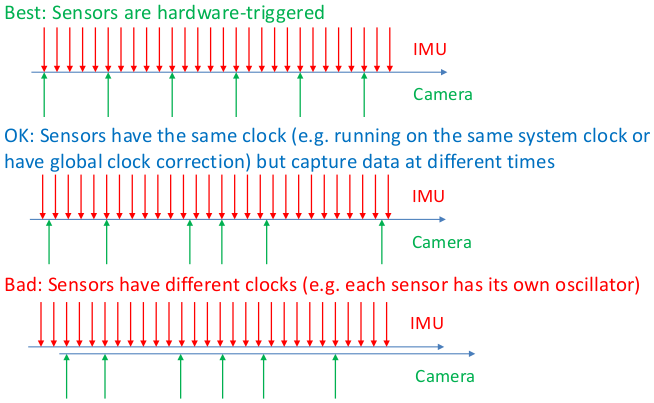
\includegraphics[scale=0.4]{images/time_synchronization.png}
\caption{Time Synchronization}
\label{fig:time_synchronization}
\end{figure}

\begin{enumerate}

\item Timestamps and Time Synchronization,如图 \ref{fig:time_synchronization}

\begin{itemize}
  \item Timestamp: how the time for each sensor measurement is tagged
  \item Best: timestamping is done at data capture
  \item OK: fixed latency for time stamping
  \item Bad: variable latency in time stamping
\end{itemize}

\item Temporal Calibration

\begin{itemize}
\item calibrate the fixed latency $t_d$ occurred during time stamping
\item change the IMU pre-integration interval to the interval between two image timestamps
  \begin{itemize}
  \item linear incorporation of IMU measurements to obtain the IMU reading at image time stamping
  \item estimates states(position, orientation, etc.) at image time stamping
  \end{itemize}
\end{itemize}

\item Vision measurement residual for temporal calibration \cite{qin2018online}

\begin{itemize}

\item Feature velocity on image plane

feature l moves at speed $V_l^k$ from image k to $k+1$ in short time period $[t_k,t_{k+1}]$

\begin{equation}
\mathbf{V}_{l}^{k}=\left(\left[\begin{array}{c}{u_{l}^{k+1}} \\ {v_{l}^{k+1}}\end{array}\right]-\left[\begin{array}{c}{u_{l}^{k}} \\ {v_{l}^{k}}\end{array}\right]\right) /\left(t_{k+1}-t_{k}\right)
\end{equation}

\item Visual measurement residual with time offset

New state variable $t_d$, and estimate states $(c^{i'}, c^{j'})$ at time stamping

\begin{equation}
\begin{aligned} 
\mathbf{e}_{l}^{j} &=
\mathbf{z}_{l}^{j}\left(t_{d}\right)-\pi\left(\mathbf{R}_{c_{i}}^{w^{T}}\left(\mathbf{R}_{c_{j}}^{w} \lambda_{i}\left[\begin{array}{c}{\mathbf{z}_{l}^{i}\left(t_{d}\right)} \\ {1}\end{array}\right]+\mathbf{p}_{c_{i}}^{w}-\mathbf{p}_{c_{j}}^{w}\right)\right) \\ 
\mathbf{z}_{l}^{i} &=\left[u_{l}^{i} v_{l}^{i}\right]^{T}+t_{d} \mathbf{V}_{l}^{i}, \quad 
\mathbf{z}_{l}^{j}=\left[u_{l}^{j} v_{l}^{j}\right]^{T}+t_{d} \mathbf{V}_{l}^{j} 
\end{aligned}
\end{equation}

\end{itemize}

视觉残差和雅克比矩阵计算的对应代码在 \verb|ProjectionTdFactor::Evaluate| 函数中。

\begin{lstlisting}
// TR / ROW * row_i 是相机 rolling 到这一行时所用的时间
Eigen::Vector3d pts_i_td, pts_j_td;
pts_i_td = pts_i - (td - td_i + TR / ROW * row_i) * velocity_i;
pts_j_td = pts_j - (td - td_j + TR / ROW * row_j) * velocity_j;

Eigen::Vector3d pts_camera_i = pts_i_td / inv_dep_i;
Eigen::Vector3d pts_imu_i    = qic * pts_camera_i + tic;
Eigen::Vector3d pts_w        = Qi * pts_imu_i + Pi;
Eigen::Vector3d pts_imu_j    = Qj.inverse() * (pts_w - Pj);
Eigen::Vector3d pts_camera_j = qic.inverse() * (pts_imu_j - tic);

Eigen::Map<Eigen::Vector2d> residual(residuals);
#ifdef UNIT_SPHERE_ERROR
residual =  tangent_base * (pts_camera_j.normalized() - pts_j_td.normalized());
#else
double dep_j = pts_camera_j.z();
residual = (pts_camera_j / dep_j).head<2>() - pts_j_td.head<2>();
#endif
residual = sqrt_info * residual;
\end{lstlisting}

添加对 imu-camera 时间戳不完全同步和 Rolling Shutter 相机的支持:通过前端光流计算得到每个角点在归一化的速度,根据 imu-camera 时间戳的时间同步误差和Rolling Shutter相机做一次rolling的时间,对角点的归一化坐标进行调整

\end{enumerate}

\subsection{边缘化(Marginalization)}

\begin{quote}
SLAM is tracking a noraml distribution through a large state space.
\end{quote}

\begin{figure}[htbp]
\centering
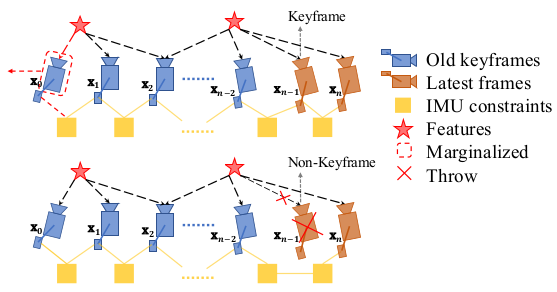
\includegraphics[scale=0.6]{images/marginalization.png}
\end{figure}

\textbf{滑窗(Sliding Window)} 限制了关键帧的数量,防止pose和feature的个数不会随时间不断增加,使得优化问题始终在一个有限的复杂度内,不会随时间不断增长。

\subsubsection{Marginalization}

然而,将pose移出windows时,有些约束会被丢弃掉,这样势必会导致求解的精度下降,而且当MAV进行一些退化运动(如: 匀速运动)时,没有历史信息做约束的话是无法求解的。所以,在移出位姿或特征的时候,需要将相关联的约束转变成一个约束项作为prior放到优化问题中,这就是marginalization要做的事情。

边缘化的过程就是将滑窗内的某些较旧或者不满足要求的视觉帧剔除的过程,所以边缘化也被描述为\textbf{将联合概率分布分解为边缘概率分布和条件概率分布的过程}(就是\textbf{利用shur补减少优化参数}的过程)。

直接进行边缘化而不加入先验条件的后果:

\begin{enumerate}
\item 无故地移除这些pose和feature会丢弃帧间约束,会降低了优化器的精度,所以在移除pose和feature的时候需要将相关联的约束转变为一个先验的约束条件作为prior放到优化问题中

\item 在边缘化的过程中,不加先验的边缘化会导致系统尺度的缺失(参考[6]),尤其是系统在进行退化运动时(如无人机的悬停和恒速运动)。一般来说 \textbf{只有两个轴向的加速度不为0的时候,才能保证尺度可观},而退化运动对于无人机或者机器人来说是不可避免的。所以在系统处于退化运动的时候,要加入先验信息保证尺度的可观性
\end{enumerate}

VINS-Mono中为了处理一些悬停的case,引入了一个two-way marginalization:

\begin{enumerate}
\item \verb|MARGIN_OLD|:如果次新帧是关键帧,则丢弃滑动窗口内最老的图像帧,同时对与该图像帧关联的约束项进行边缘化处理。这里需要注意的是,如果该关键帧是观察到某个地图点的第一帧,则需要把该地图点的深度转移到后面的图像帧中去。

\item \verb|MARGIN_NEW|:如果次新帧不是关键帧,则丢弃当前帧的前一帧。因为判定当前帧不是关键帧的条件就是当前帧与前一帧视差很小,也就是说当前帧和前一帧很相似,这种情况下直接丢弃前一帧,然后用当前帧代替前一帧。为什么这里可以不对前一帧进行边缘化,而是直接丢弃,原因就是当前帧和前一帧很相似,因此当前帧与地图点之间的约束和前一帧与地图点之间的约束是很接近的,直接丢弃并不会造成整个约束关系丢失信息。这里需要注意的是,要把当前帧和前一帧之间的 IMU 预积分转换为当前帧和前二帧之间的 IMU 预积分。

\end{enumerate}

在悬停等运动较小的情况下,会频繁的 \verb|MARGIN_NEW|,这样也就保留了那些比较旧但是视差比较大的pose。这种情况如果一直 \verb|MARGIN_OLD| 的话,视觉约束不够强,状态估计会受IMU积分误差影响,具有较大的累积误差。

\subsubsection{Schur Complement}

Marginalization via Schur complement on information matrix

\begin{figure}[htbp]
\centering
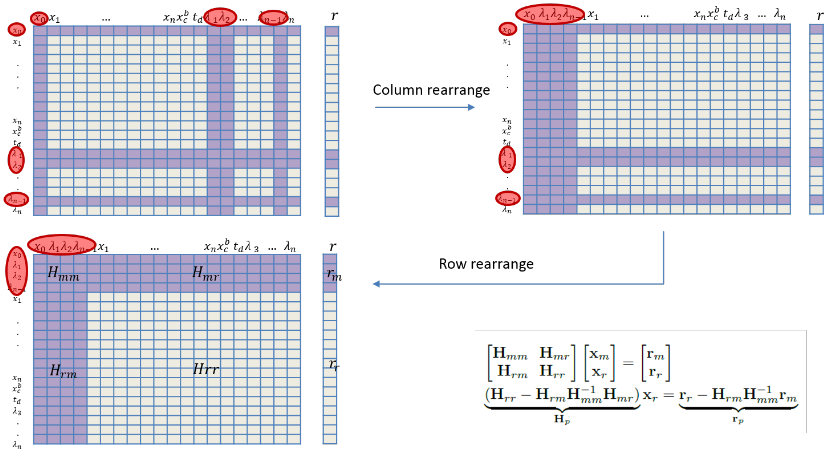
\includegraphics[scale=0.5]{images/schur_complement.png}
\end{figure}

\subsubsection{First Estimate Jacobin}

\section{重定位}

\subsection{Loop Detection}

Vins-Mono利用 词袋 DBoW2 做Keyframe Database的构建和查询。在建立闭环检测的数据库时,关键帧的Features包括两部分:VIO部分的200个强角点 和 500个Fast角点,然后描述子使用 BRIEF (因为旋转可观,匹配过程中对旋转有一定的适应性,所以不用使用ORB)。

\begin{enumerate}
\item Describe features by BRIEF
  \begin{enumerate}
  \item Features that we use in the VIO (200, not enough for loop detection)
  \item Extract new FAST features (500, only use for loop detection)
  \end{enumerate}
\item Query Bag-of-Word (DBoW2)
  \begin{enumerate}
  \item Return loop candidates
  \end{enumerate}
\end{enumerate}

\subsection{Feature Retrieval}

在闭环检测成功之后,会得到回环候选帧,所以要在已知位姿的回环候选帧和滑窗内的匹配帧通过\textbf{BRIEF描述子匹配},然后把回环帧加入到滑窗的优化当中,这时整个滑窗的状态量的维度是不发生变化的,因为回环帧的位姿是固定的。

\begin{enumerate}
\item Try to retrieve matches for features (200) that are used in the VIO
\item BRIEF descriptor match
\item Geometric check
  \begin{enumerate}
  \item 2D-2D: fundamental matrix test with RANSAC
  \item 3D-3D: PnP test with RANSAC
  \item At least 30 inliers
  \end{enumerate}
\end{enumerate}

\subsection{Tightly-Coupled Relocalization}

\section{全局位姿图优化}

因为之前做的非线性优化本质只是在一个滑窗之内求解出了相机的位姿,而且在回环检测部分,利用固定位姿的回环帧只是纠正了滑窗内的相机位姿,并没有修正其他位姿(或者说没有将回环发现的误差分配到整个相机的轨迹上),缺少全局的一致性,所以要做一次全局的Pose Graph。\textbf{全局的Pose Graph较之滑窗有一定的迟滞性,只有相机的Pose滑出滑窗的时候,Pose才会被加到全局的Pose Graph当中。}

\begin{enumerate}
\item Adding Keyframes into the Pose Graph

\begin{enumerate}
\item Sequential edges from VIO
  \begin{enumerate}
  \item Connected with 4 previous keyframes
  \end{enumerate}
\item Loop closure edges
  \begin{enumerate}
  \item Only added when a keyframe is marginalized out from the sliding window VIO
  \item Multi-constraint relocalization helps eliminating false loop closures
  \item Huber norm for rejection of wrong loops
  \end{enumerate}
\end{enumerate}

\item 4-DOF Pose Graph Optimization

\begin{enumerate}
\item Roll and pitch are observable from VIO
\end{enumerate}

\item Pose Graph Management

\item Map Reuse

\begin{enumerate}
\item Save map at any time
\item Load map and re-localize with respect to it
\item Pose graph merging
\end{enumerate}

\end{enumerate}

\section{Remarks on Monocular Visual-Inertial SLAM}

\begin{enumerate}
\item Important factors
  \begin{enumerate}
  \item Access to raw camera data (especially for rolling shutter cameras)
  \item Sensor synchronization and timestamps
  \item Camera-IMU rotation
  \item Estimator initialization
  \end{enumerate}
\item Not-so-important factors
  \begin{enumerate}
  \item Camera-IMU translation
  \item Types of features (we use the simplest corner+KLT)
  \item Quality of feature tracking (outlier is acceptable)
  \end{enumerate}
\item Failures – need more engineering treatment
  \begin{enumerate}
  \item Long range scenes (aerial vehicles)
  \item Constant velocity (ground vehicle)
  \item Pure rotation (augmented reality)
  \end{enumerate}
\item Be aware of computational power requirement
\end{enumerate}

\bibliography{bibfile}

\printindex

\end{document}